\documentclass[12pt,a4paper,twoside]{article}
\usepackage{labor}
\begin{document}

%fill for cover and header creation
\newcommand\laboratorynumber{2}
\title{Gitter/Prisma}
\newcommand\supervisor{Weis, Valentin}
\newcommand\groupnumber{42}

\newcommand\participantonelastname{Eisner}
\newcommand\participantonefirstname{Nico}
\newcommand\participantoneid{12214121}
\newcommand\participanttwolastname{Waldl}
\newcommand\participanttwofirstname{Philip}
\newcommand\participanttwoid{12214120}
\author{\participantonelastname \ \& \participanttwolastname}

\newcommand\degreeid{UB 033 678}
\newcommand\semester{23WS}
\date{13.10.2023}

%select correct course title
%\newcommand\coursetitle{Einführung in die \\ physikalischen Messmethoden}
%\newcommand\coursetitle{Laborübungen 1: \\ Mechanik und Wärme}
\newcommand\coursetitle{Laborübungen 2: \\ Elektrizität, Magnetismus, Optik}
%\newcommand\coursetitle{Fortgeschrittenen Praktikum 1: \\ Technische Physik}
%\newcommand\coursetitle{Fortgeschrittenen Praktikum 2: \\ Allgemeine Physik}

%\begin{titlepage}
   \begin{center}
       \begin{figure}[H]
            \begin{minipage}[h]{30mm}
                \centerline{
\includegraphics[height=15mm]{cover_nudes/tugraz.png}}
            \end{minipage}
            \hfill
            \begin{minipage}[h]{30mm}
                \centerline{
\includegraphics[height=15mm]{cover_nudes/nawi_graz.png}}
            \end{minipage}
            \hfill
            \begin{minipage}[h]{30mm}
                \centerline{
\includegraphics[height=15mm]{cover_nudes/uni-graz.png}}
            \end{minipage}
        \end{figure}
        
        \large{\emph{Institut für Experimentalphysik der Technischen Universität Graz \\
        \& Institut für Physik der Universität Graz}} \\
        \vspace{5mm}
        
        {\Huge \textbf{\coursetitle}}
        \vspace{5mm}
        
        {\huge \laboratorynumber: \thetitle}
    \end{center}
    
    \vfill
    
    \begin{table}[H]
        \LARGE
        \centering
        \begin{tabular}{r l}
            Betreuer:       & \supervisor \\
            Gruppennummer:  & \groupnumber \\
            \\
            Name:           & \participantonelastname, \participantonefirstname \\
            Matrikelnummer: & \participantoneid \\
            Name:           & \participanttwolastname, \participanttwofirstname \\
            Matrikelnummer: & \participanttwoid \\
            \\
            Kennzahl:       & \degreeid \\
            Datum:          & \semester \ | \thedate
        \end{tabular}
    \end{table}
    \vspace{4cm}
\end{titlepage}
\clearpage
\setcounter{page}{1}

%\maketitle %short title alternative

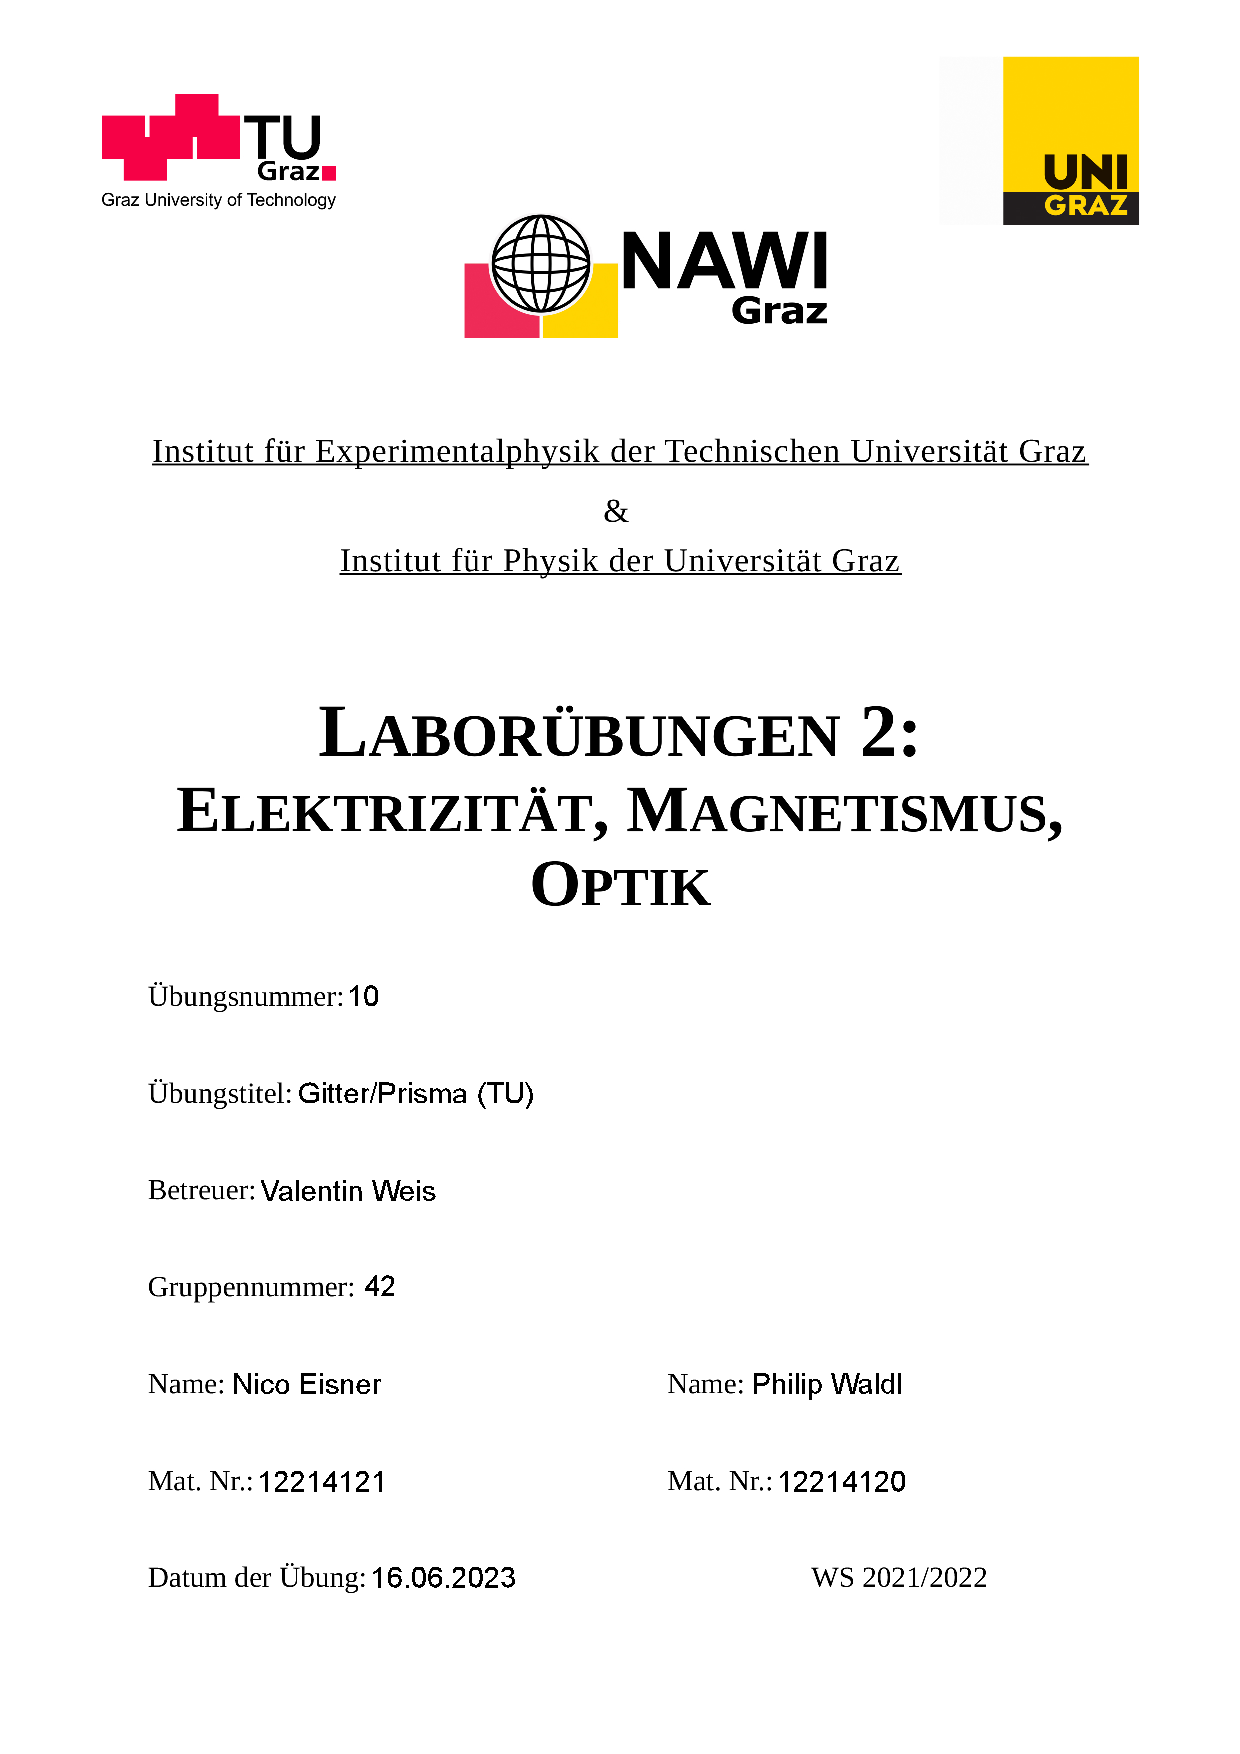
\includepdf[pages={1}]{../Deckblätter/Deckblatt_Gitter.pdf}

\tableofcontents
\newpage

\section{Aufgabenstellung} %jo beschreibn wos gmocht host ------------------------------
Das Experiment Gitter/Prisma ist in zwei Teile gegliedert. Die Aufgabe beim Gitter ist es, die Gitterkonstante $g$ mithilfe einer gelben Na-Dampflampe zu bestimmen, sowie die Wellenlänge $\lambda$ der sichtbaren Linien einer Spektrallampe. 
\\
Im zweiten Teil des Experimentes besteht die Aufgabe den brechenden Winkel eines Prismas $\gamma$ durch Messung des Reflexionswinkels $\omega$ zu bestimmen. 
Des weiteren ist auch der minimale Brechungswinkel $\delta$ sowie der Brechungsindex $n(\lambda_0)$ des Prismas für die gut sichtbaren Linien einer Hg-Dampflampe zu bestimmen. 
\\
\\
Alle Informationen und Methodiken wurden uns von der Technischen Universität bereitgestellt \cite{teachcenter2}. 

\section{Voraussetzungen \& Grundlagen} %Grundlagen erklären, Formeln mit erklärung
\subsection{Gitter}
Ein Gitter besteht aus lichtdurchlässigen Öffnungen und lichtblockenden Balken, welche in bestimmten Abständen folgen. Ein Beispiel für ein Gitter aus dem Alltag ist eine CD. 
In diesem Fall besteht das Gitter aus einer Glasplatte. Fällt Licht auf dieses Gitter, wird es gebeugt und von jeden Punkt einer Öffnung gehen Kugelförmige Lichtwellen aus, welche sich nach Richtung und Wellenlänge durch Interferenzen verstärken oder abschwächen. 
\\
\\
%Bild
\\
Durch viele aufeinanderfolgende Balken in regelmäßigen Öffnungsabständen $g$ (Gitterkonstante) können alle neuen Wellen interferieren. Dabei tritt je nach Winkel $\varphi$ eine konstruktive oder destruktive Interferenz auf. 
Die konstruktiven Interferenzen können als Beugungsmaxima der Wellenlänge $\lambda$ beobachtet werden. 

    \begin{equation}
        \label{eq:Gitterkonstante}
        \centerline{$\Delta=g sin(\varphi) = z\lambda$,     $z \in \mathbb{Z} $}
    \end{equation}

\noindent
Die Zahl $z$ ist die Ordnungszahl des Beugungsmaximums. 
\\
\\
Das Auflösungsvermögen $\Delta \lambda / \lambda$ des Gitters wird über die Größe $D/g$ berechnet, welche die Anzahl $N$ aller vom Licht getroffenen Gitterstriche darstellt.  

\begin{equation}
    \label{eq:Auflösungsvermögen}
    \centerline{$\frac{\lambda}{\Delta \lambda} = zN = \frac{zD}{g}$}
\end{equation}

\subsection{Prisma}
Licht wird durch einen Prisma gebrochen. 
Die Bahn eines einfarbigen Lichtstrahls einer Frequenz durch verschiedene Medien wird eindeutig festgelegt. Die entscheidenden Faktoren sind dabei die Brechungsindizes der verschiedenen Medien, die geometrische Form und Lage ihrer Begrenzungsflächen. 
Reflektionen und Brechungen treten an der Grenze zweier Medien mit verschiedenen Brechungsindizes auf. Der Einfallende Strahl $E$ wird im selben Winkel $\alpha$ mit dem Lot $L$ wieder Reflektiert $R$. 
Der Winkel $\beta$ zwischen gebrochenen Strahl $G$ und Lot $L$ wird mithilfe des Brechungsgesetzes von Snellius berechnet. 

\begin{equation}
    \label{eq:Snellius}
    \centerline{$sin(\alpha) n_1 = sin(\beta) n_2$}
\end{equation}

\begin{figure}[H]
    \centering
    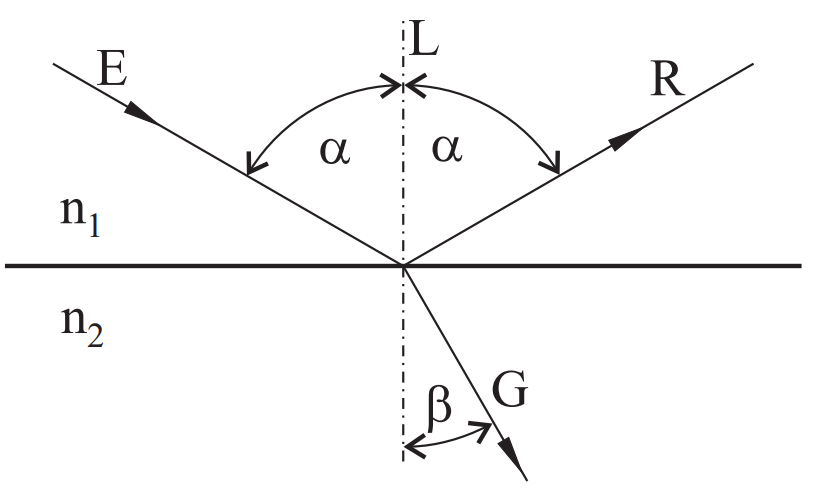
\includegraphics[width=0.6\linewidth]{nudes/Brechung.png}
    \caption{Brechung und Reflexion an einen Übergang. \cite{teachcenter2}}
    \label{fig:brechung}
\end{figure}

\noindent
Bei einen Strahlengang durch den Prisma wird das Licht zwei mal gebrochen. 
Das Licht ändert seine Richtung unter dem Ablenkungswinkel $\delta $ bei einem symmetrischen Strahlengang. Hierbei ist der Ein- und Austrittswinkel gleich groß. 
Dieser Winkel kann durch schwenken des Prismas leicht gefunden werden. 
Misst man nun den Winkel $\omega$ zwischen zwei zum einfallenden Strahl symmetrischen Lagen des Prismas, kann der Ablenkungswinkel $\delta $ berechnet werden. 

\begin{equation}
    \label{eq:Ablenkungswinkel}
    \centerline{$\delta = \omega /2$}
\end{equation}

\noindent
Formt man nun die Gleichung auf den Brechungsindex $n$ des Prismas um, so erhält man

\begin{equation}
    \label{eq:Brechungsindex}
    \centerline{$ n = \frac{sin(\frac{\gamma + \delta }{2})}{sin(\gamma /2)}$}
\end{equation}
dies lässt sich jedoch nur bei symmetrischen Strahlengang bewerkstelligen. 
\\
\\
Um das Auflösungsvermögen eines Prismas zu berechnen, benötigt man den Brechungsindex $n$, sowie die Wellenlänge $\lambda$. Der Wert $t$ ist die Basislänge des wirksamen Strahlenbündels im Prisma. $D$ wird als Dispersion bezeichnet. 
\begin{equation}
    \label{eq:Auflösungsvermögen Prisma}
    \centerline{$\frac{\lambda}{\Delta \lambda} = tD = t \frac{dn}{d \lambda}$}
\end{equation}
\\
\\
Desweiteren wird die Formel für die Berechnung des Mittelwertes der verschiedenen Spektrallinien benötigt. Um den Mittelwert \={x} (representativ für die verschiedenen Winkel) zu berechnen, müssen die Anzahl der Messversuche N sowie die einzelnen Winkel bekannt sein. 
\begin{equation}
    \label{eq:Mittelwert}
    \centerline{$\bar{x} = \frac{1}{N} \sum_{i = 1}^{N} x_i $}
\end{equation}

\section{Versuchsanordnung} %mit skizze kurz beschreiben ------------------------------
Der Aufbau des Versuches mit dem Gitter ist wiefolgt. Es besteht aus einen Spektrometertisch. Dieser ist in Kollimator, einen Fernrohr auf einer rotierbaren Winkelskala und einer Ablage für Gitter und Prisma in der Mitte. 
Die Lichtquellen sind eine Quecksilberlampe und eine Natriumlampe, welche je nach Versuch an die Öffnung des Kollimators gestellt. 
Durch die in den Kollimator verbaute Schlitzblende wird die Stärke bzw. Helligkeit des Lichtstrahles eingestellt. 
Das Licht, welches durch den Kollimator parallelisiert wird, trifft auf das Gitter, im späteren Verlauf auf den Prisma, und wird dort gebrochen/gebeugt. 
Mit dem Fernrohr lässt sich das Licht nun beobachten und durch das Fadenkreuz kann ein einzelner Strahl genauestens anvisiert werden. 

    \begin{figure}[H]
        \centering
        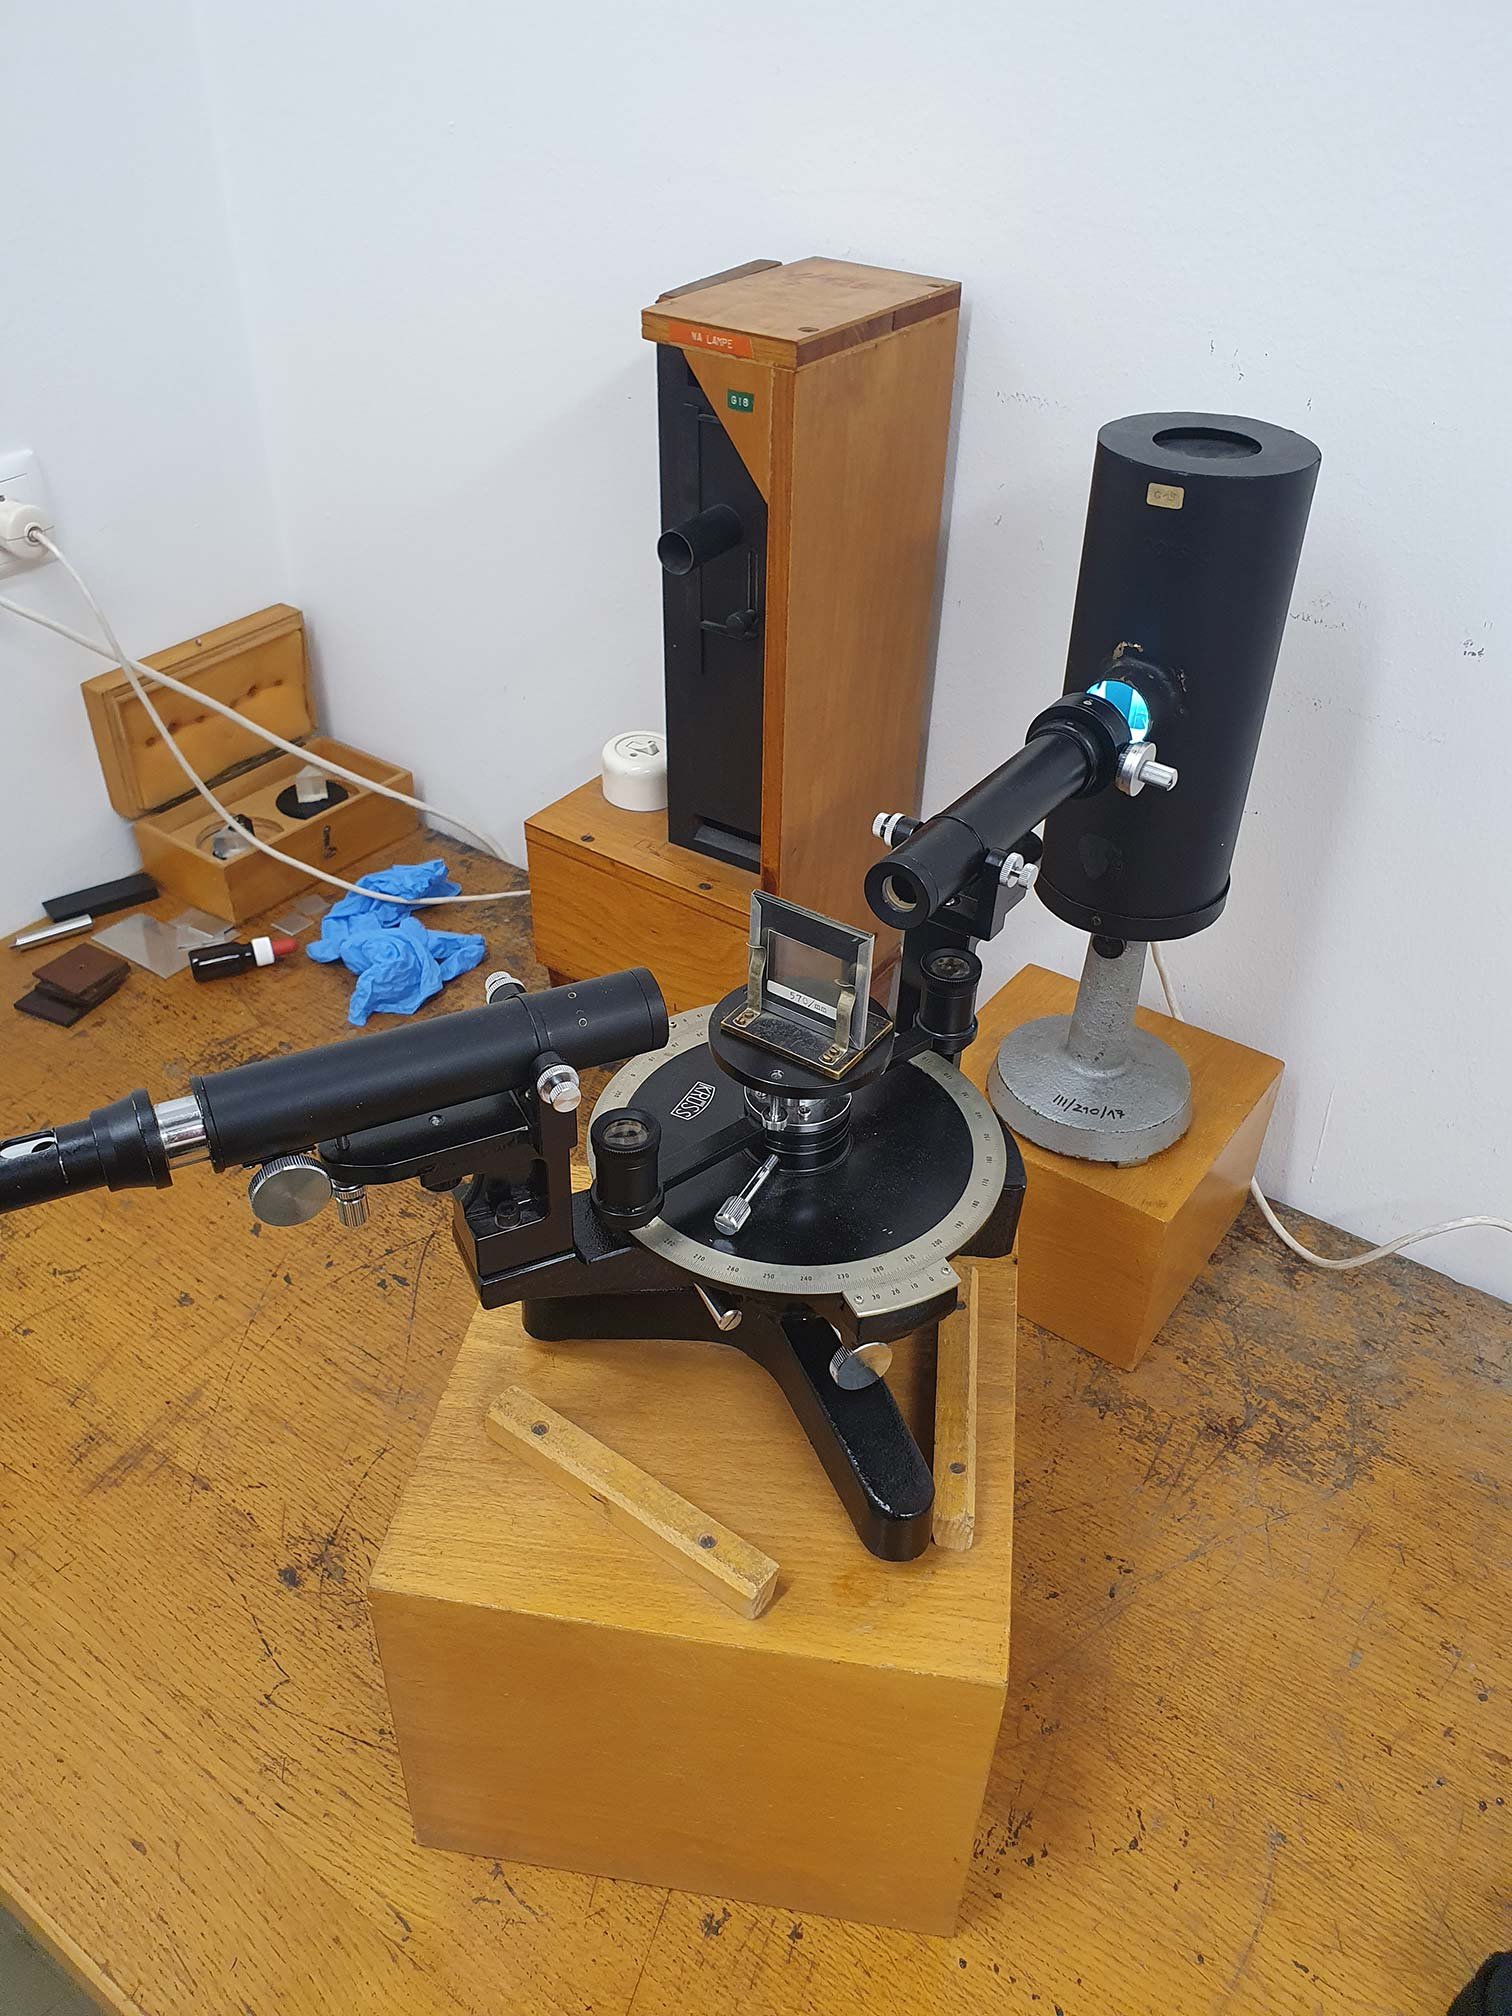
\includegraphics[width=0.6\linewidth, angle=-90]{nudes/versuch.jpg}
        \caption{Aufbau des Spektrometertisches}
        \label{fig:Aufbau}
    \end{figure}
\noindent
Das Fernrohr wird für die Messung des Winkels nach links und rechts gescwenkt und auf der Winkelskala der entsprechende Winkel abgelesen. 

\begin{figure}[H]
    \centering
    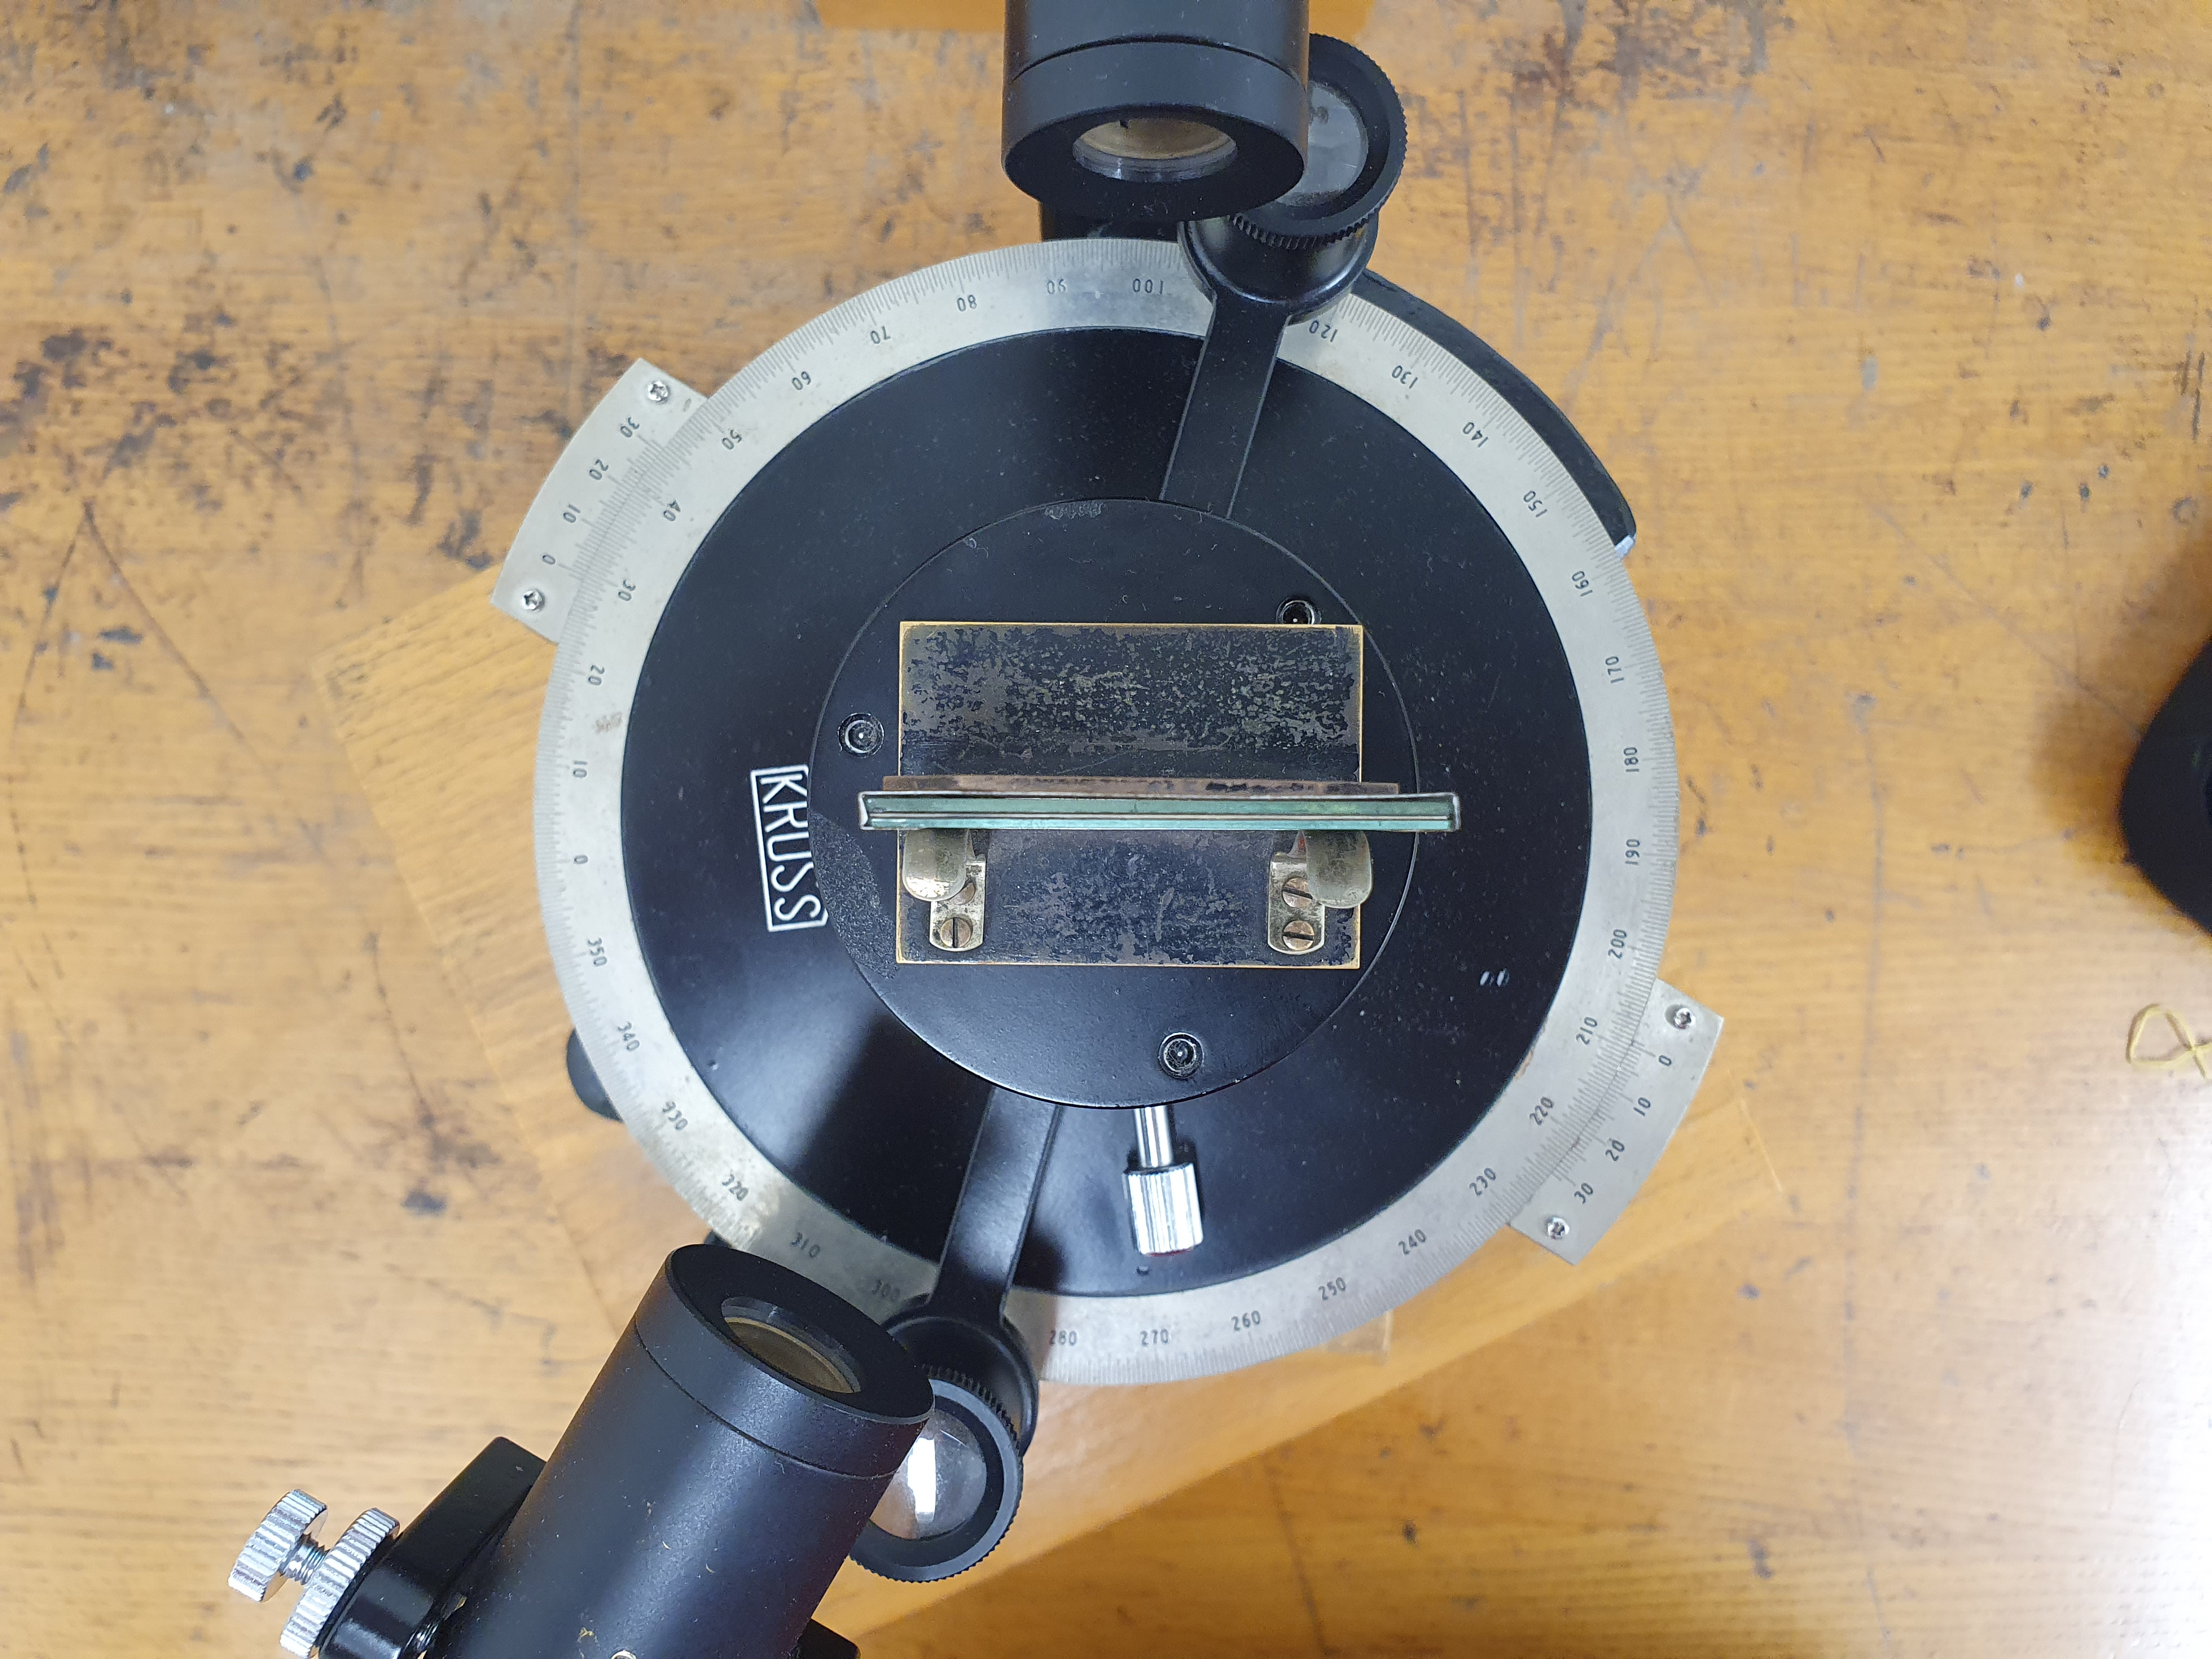
\includegraphics[width=0.6\linewidth, angle=-90]{nudes/messskala.jpg}
    \caption{Winkelskala}
    \label{fig:Winkelskala}
\end{figure}

\begin{figure}[H]
    \centering
    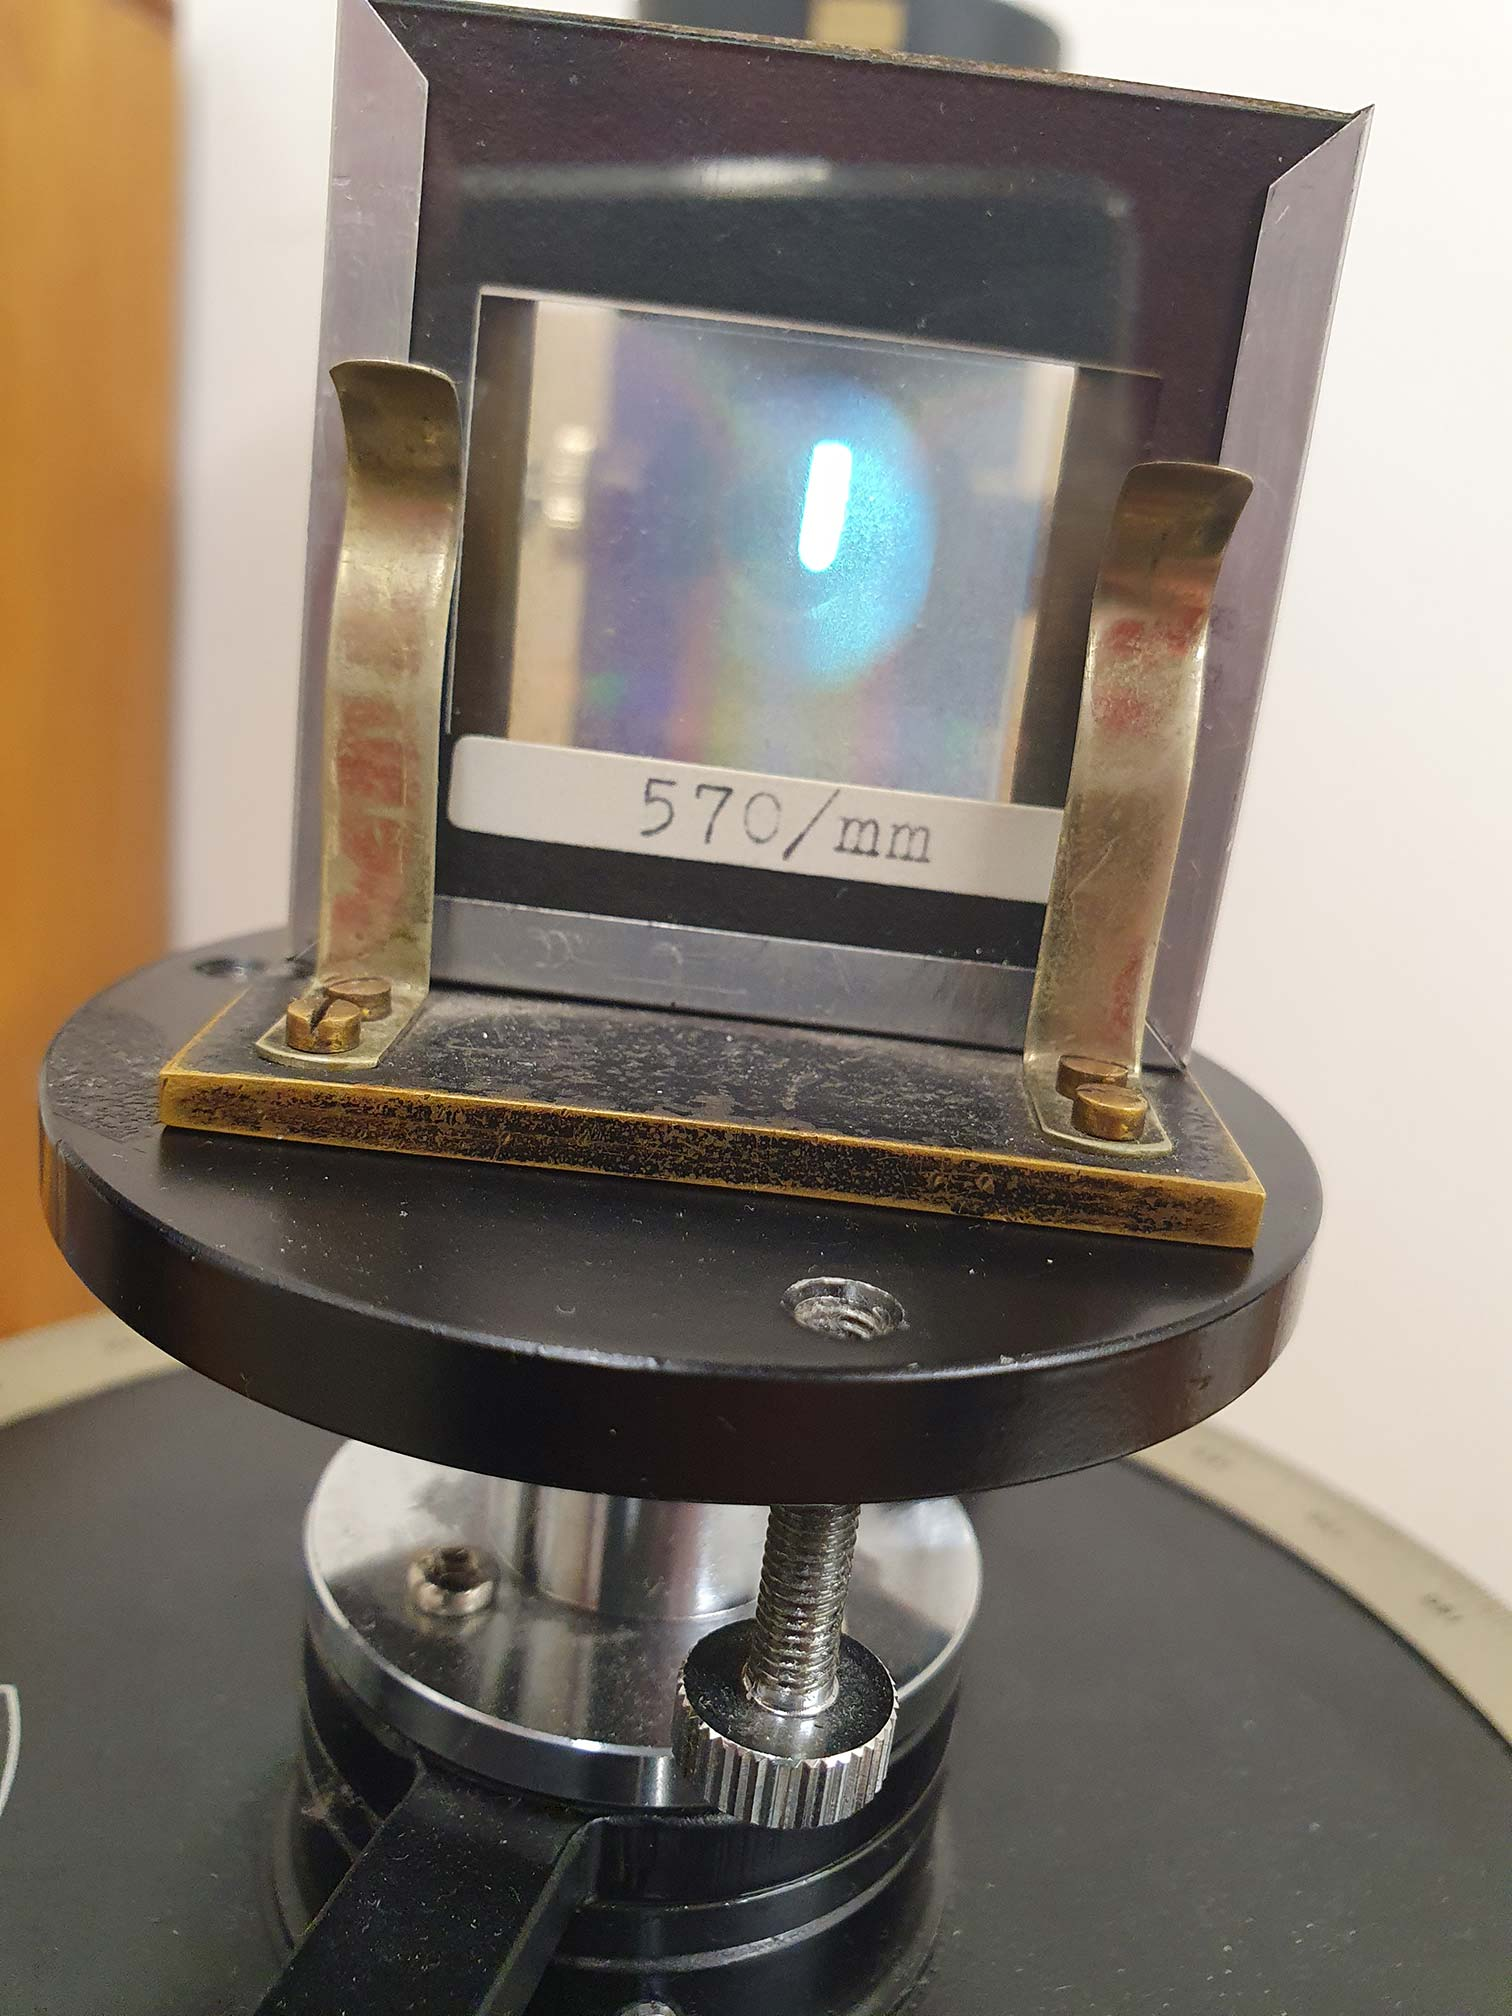
\includegraphics[width=0.6\linewidth, angle=-90]{nudes/gitter.jpg}
    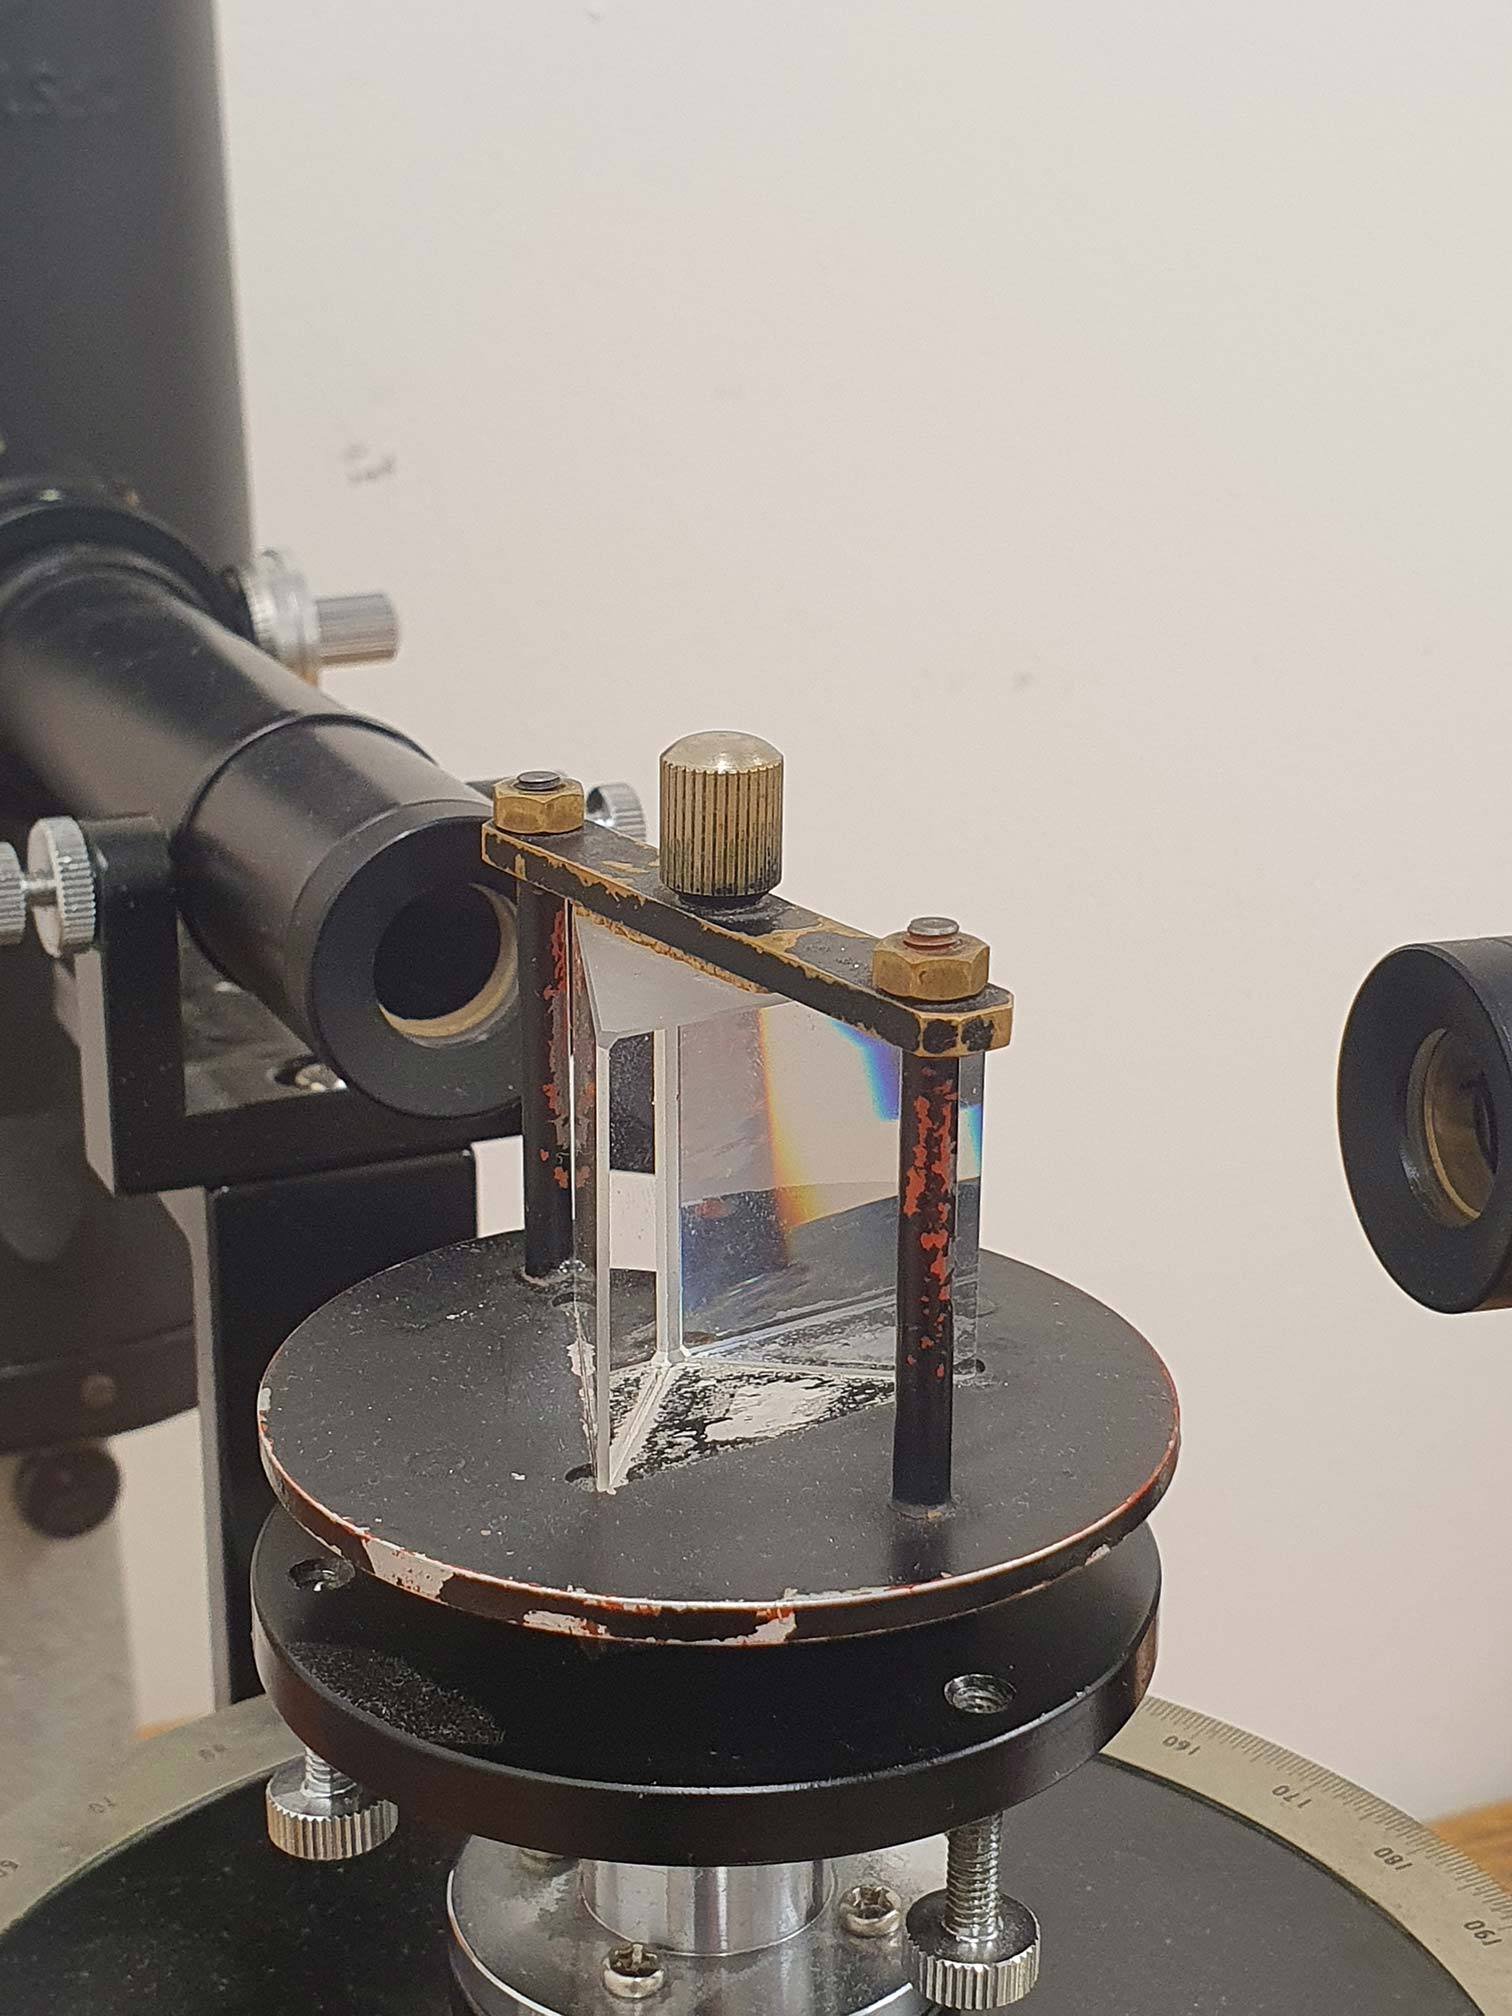
\includegraphics[width=0.6\linewidth, angle=-90]{nudes/prisma.jpg}
    \caption{Gitter (links) und Prisma (rechts)}
    \label{fig:gitterundprisma}
\end{figure}    


\section{Geräteliste} %jo holt a listn ------------------------------

    \begin{table}[H]
        \centering
        \caption{Im Versuch verwendete Geräte und Utensilien.}
        \label{tab:geraete}
        \begin{tabular}{| l | l | l |}
            \hline
            Gerät  & Gerätenummer  & Unsicherheit \\
            \hline
            Quecksilberlampe & G15 & {n.a} \\
            Natriumlampe & G18 & {n.a} \\
            Gitter 570/mm & {n.a} & {n.a} \\
            Prisma & {n.a} & {n.a} \\
            Spektrometertisch & 0161165 & {n.a} \\
            Winkelskala & {n.a} & 1 bogenminute \\
            Rollmeter & {n.a} & 0.3 mm \\
            \hline
        \end{tabular}
    \end{table}


\section{Versuchsdurchführung \& Messergebnisse} %nachvollziehbar und klar dargestellt ------------------------------
Die Versuchsdurchführung besteht aus mehreren Teilen für das Gitter und Prisma. 

\subsection{Gitter}

Der erste Teil besteht darin das Gitter zu Justieren. Dies war bereits der Fall und es wurde nur noch überprüft, dass keine Fehler vorhanden sind. Das Gitter wird mittig und normal zum Kollimator gestellt, wie in Bild \ref{fig:Aufbau} der Versuchsanordnung zu erkennen ist. 
Die Natriumlampe wird vor den Kollimator gestellt und die Blende so eingestellt, dass eine dünne, jedoch noch gut sichtbare Linie durch das Fernrohr zu erkennen ist. 
Durch schwenken des Fernrohres wird kontrolliert, ob zwei Maxima der Spektrallinien pro Seite sichtbar sind. 
Es werden insgesamt fünf Messungen pro Seite für die zwei hinteren Spektrallinien vorgenommen, wobei mit dem Fadenkreuz des Fernrohres die innere grüne Linie anvisiert wird. 

\begin{table}[H]
    \centering
    \caption{Winkel $\varphi$ der zweiten Spektrallinien der Natriumlampe}
    \label{tab:Gitter v1}
    \begin{tabular}{| l | l | l |}
        \hline
        Nr.  & $\varphi_{Links}$ [Grad + Bogenminute]  & $\varphi_{Rechts}$ [Grad + Bogenminute]\\
        \hline
        1 & 41 + (2 $\pm$ 1) & 140 + (0 $\pm$ 1) \\
        2 & 41 + (1 $\pm$ 1) & 139 + (5 $\pm$ 1) \\
        3 & 41 + (5 $\pm$ 1) & 139 + (5 $\pm$ 1) \\
        4 & 41 + (4 $\pm$ 1) & 139 + (4 $\pm$ 1) \\
        5 & 41 + (1 $\pm$ 1) & 139 + (5 $\pm$ 1) \\
        \hline
    \end{tabular}
\end{table}

\begin{figure}[H]
    \centering
    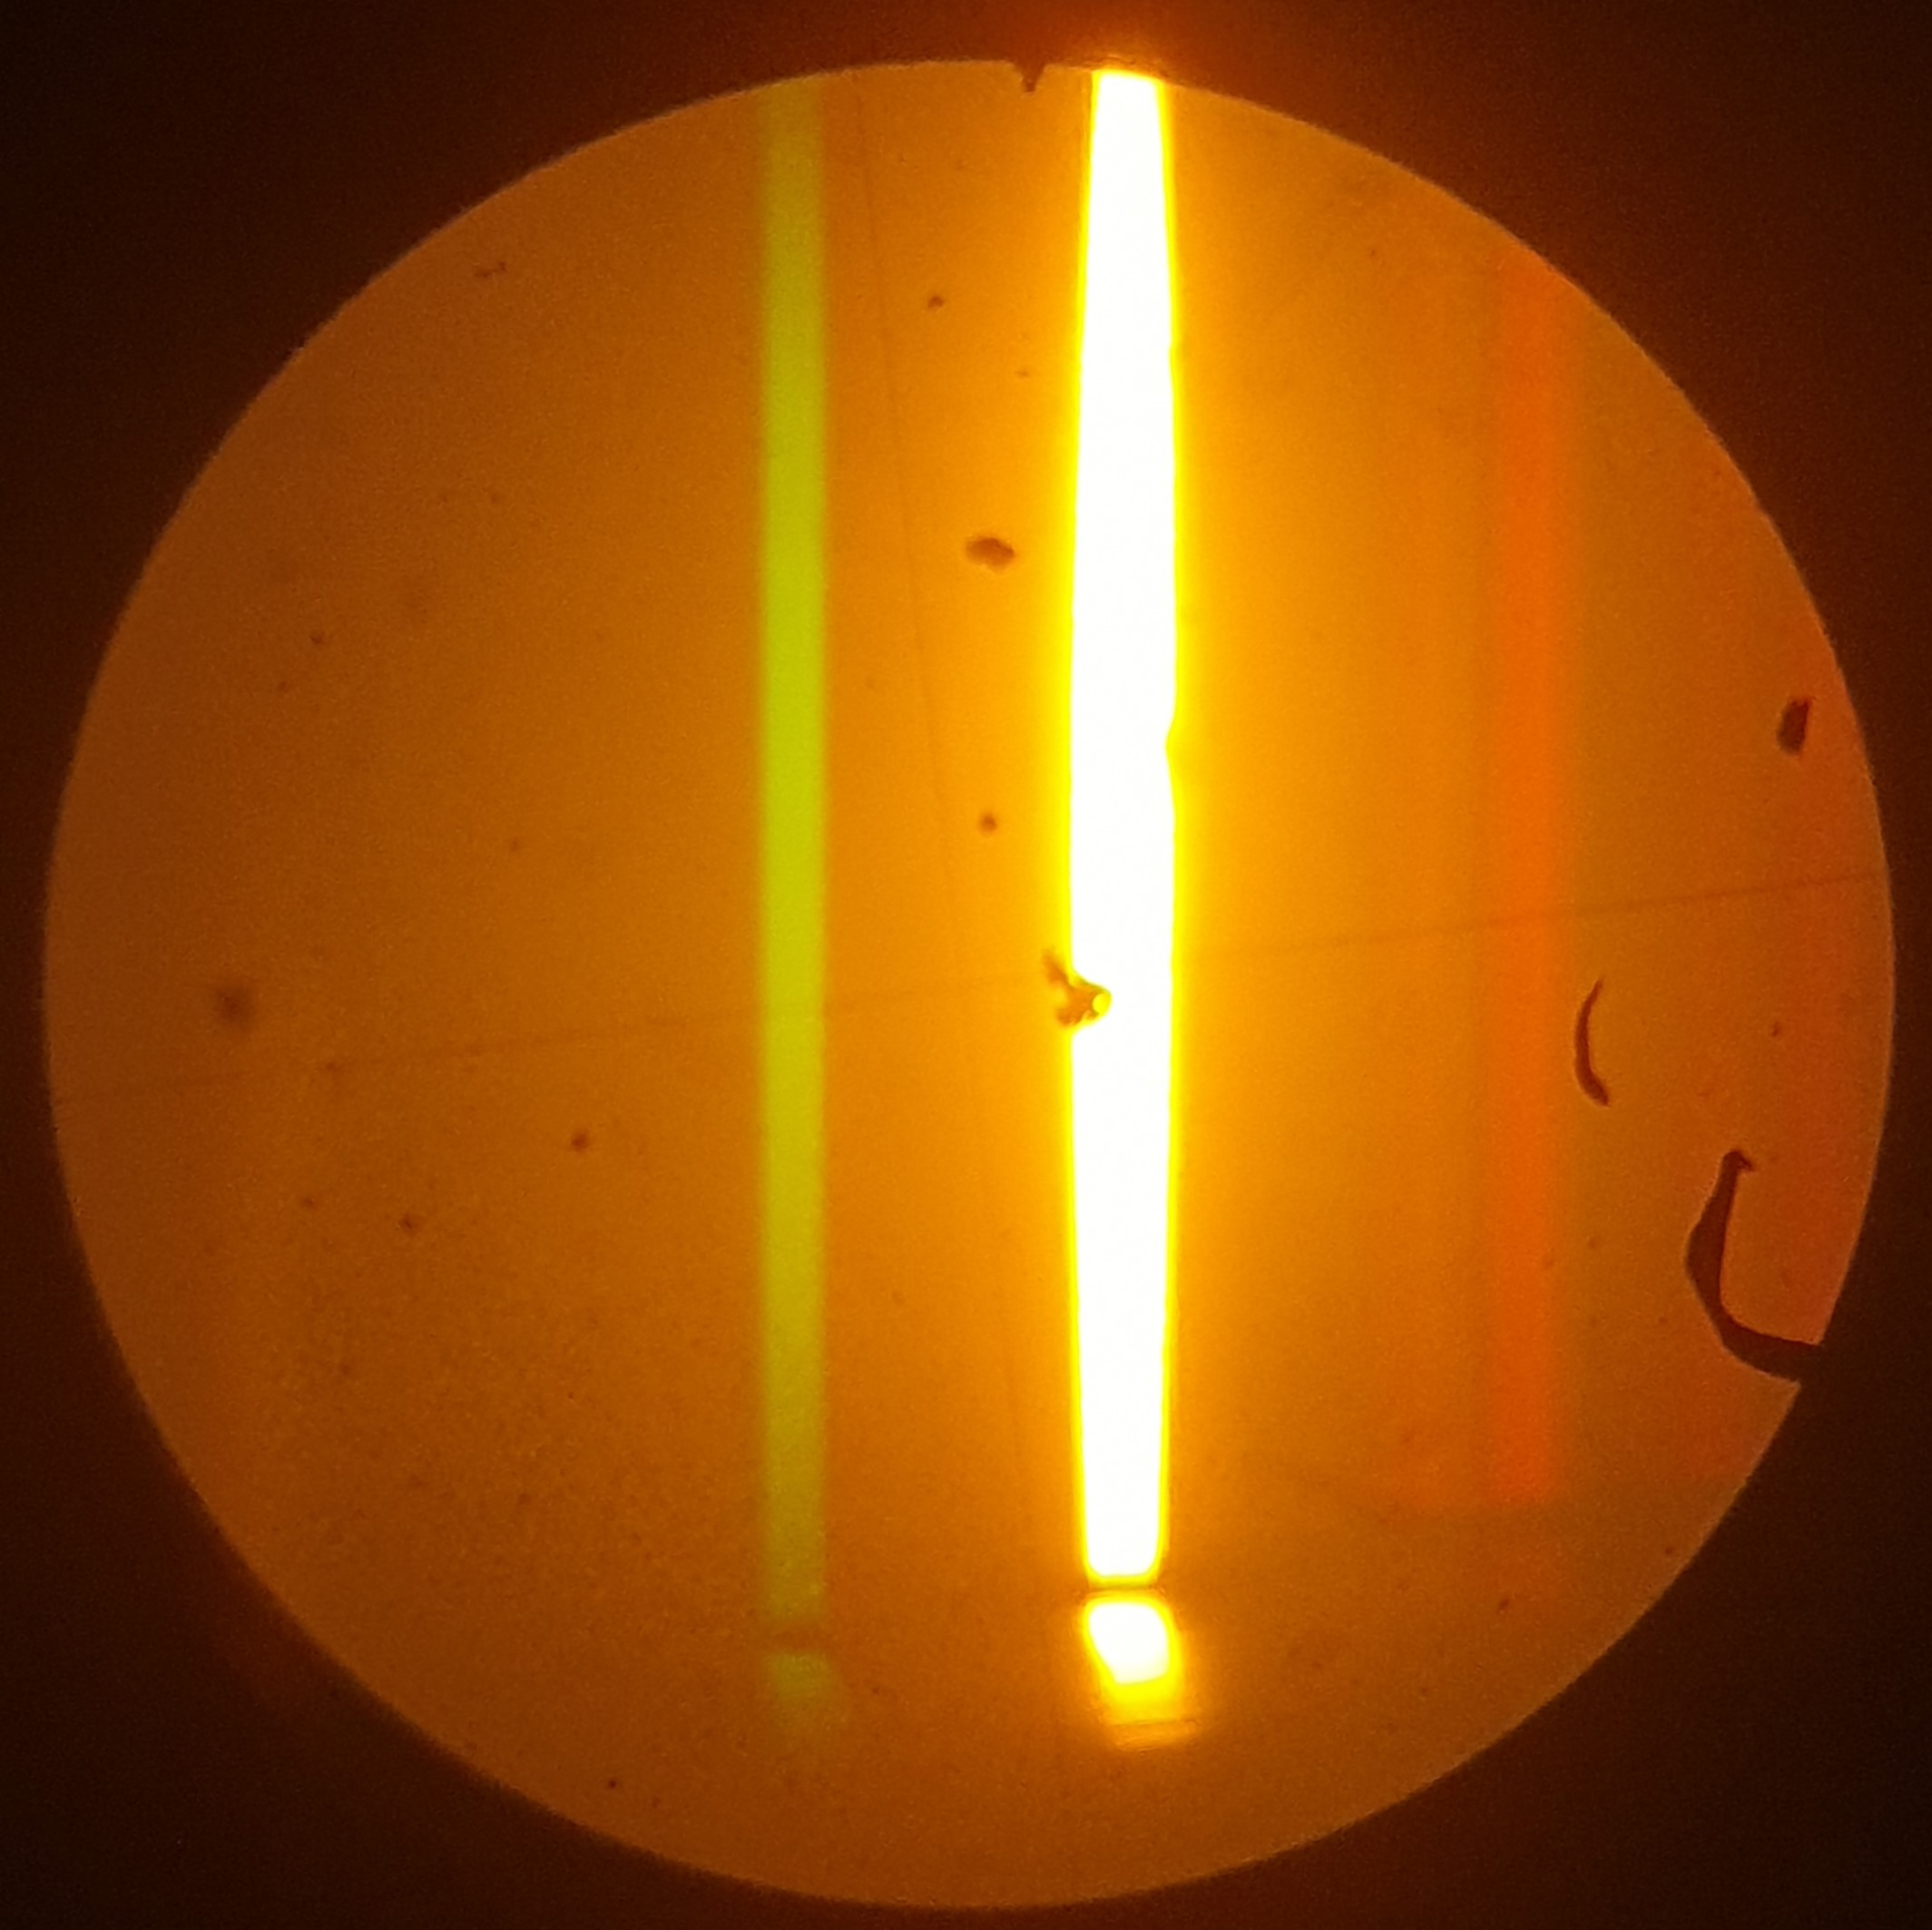
\includegraphics[width=0.6\linewidth]{nudes/na-lampe1.jpg}
    \caption{Spektrallinien der Natriumlampe bei geöffneter Blende für die Aufnahme}
    \label{fig:spektallinienNA}
\end{figure}

\noindent
Im zweiten Teil mit dem Gitter wird die Natriumlampe durch die Quecksilberlampe getauscht. 
Bei der Quecksilberlampe werden die einzelnen Wellenlängen der verschiedenfarbigen Spektrallinien gemessen. Hierbei werden wieder die zweiten hinteren Spektrallinien zur Messung genommen. 

\begin{table}[H]
    \centering
    \caption{Quecksilberlampe Gitter}
    \label{tab:Gitter v2}
    \begin{tabular}{| l | l | l | l |}
        \hline
        Farbe & Nr.  & $\varphi_{Links}$ [Grad + Bogenminute]  & $\varphi_{Rechts}$ [Grad + Bogenminute]\\
        \hline
                &  1 & 48 + (4 $\pm$ 1) & 132 + (21 $\pm$ 1) \\
        Lila     &  2 & 48 + (4 $\pm$ 1) & 132 + (20 $\pm$ 1) \\
                &  3 & 48 + (5 $\pm$ 1) & 132 + (20 $\pm$ 1) \\
        \hline
                &  1 & 41 + (17 $\pm$ 1) & 138 + (26 $\pm$ 1) \\
        Hellblau&  2 & 41 + (17 $\pm$ 1) & 138 + (26 $\pm$ 1) \\
                &  3 & 41 + (17 $\pm$ 1) & 138 + (26 $\pm$ 1) \\
        \hline
                &  1 & 36 + (0 $\pm$ 1) & 144 + (7 $\pm$ 1) \\
        Grün    &  2 & 36 + (0 $\pm$ 1) & 144 + (7 $\pm$ 1) \\
                &  3 & 36 + (1 $\pm$ 1) & 144 + (8 $\pm$ 1) \\
        \hline
                &  1 & 33 + (10 $\pm$ 1) & 146 + (20 $\pm$ 1) \\
        Gelb    &  2 & 33 + (10 $\pm$ 1) & 146 + (20 $\pm$ 1) \\
                &  3 & 33 + (11 $\pm$ 1) & 146 + (20 $\pm$ 1) \\
        \hline
                &  1 & 27 + (24 $\pm$ 1) & 155 + (5 $\pm$ 1) \\
        Rot     &  2 & 27 + (25 $\pm$ 1) & 152 + (5 $\pm$ 1) \\
                &  3 & 27 + (25 $\pm$ 1) & 152 + (5 $\pm$ 1) \\
        \hline
    \end{tabular}
\end{table}

\begin{figure}[H]
    \centering
    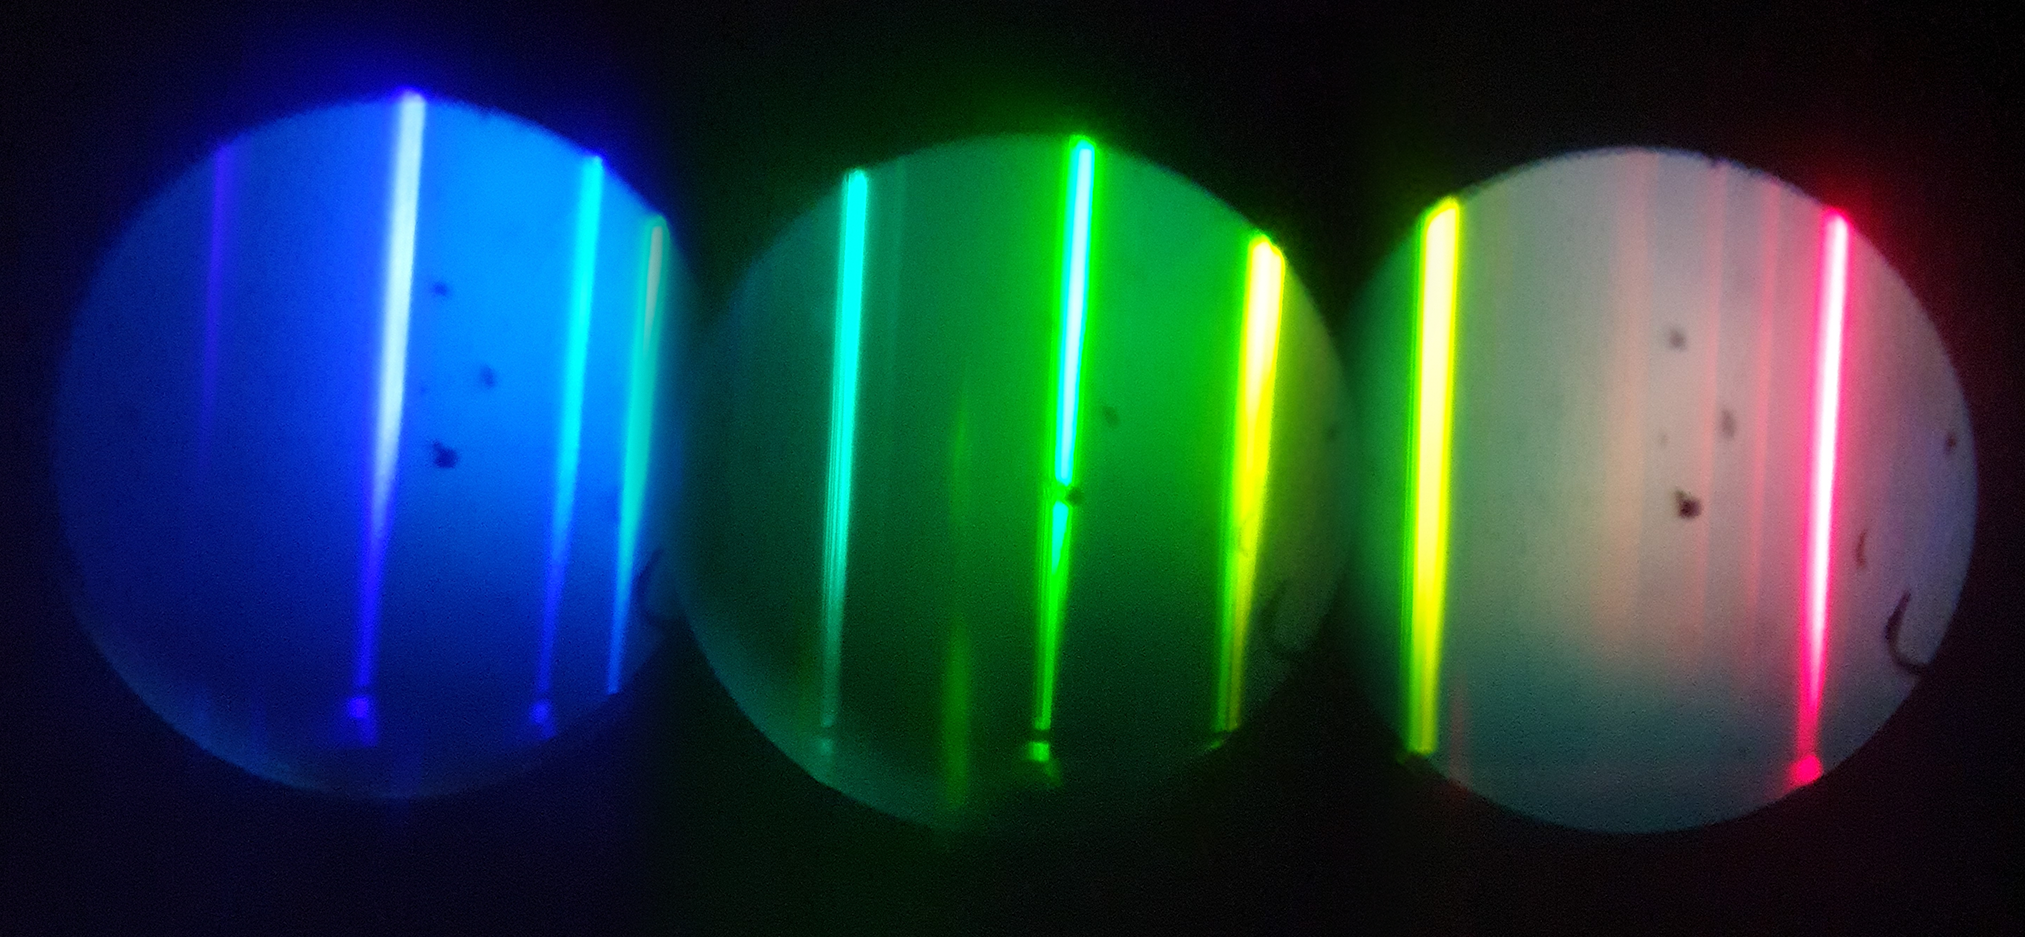
\includegraphics[width=0.6\linewidth]{nudes/stacked.png}
    \caption{Spektrallinien der einzelnen Farben der Quecksilberlampe bei geöffneter Blende für die Aufnahme. Zusammengesetzt aus drei Einzelaufnahmen.}
    \label{fig:spektallinienHG}
\end{figure}

\subsection{Prisma}
Im zweiten Teil des Experimentes wird das Gitter durch einen Prisma getauscht. 
Dieser wird mittels Augenmaß mittig auf der Ablage plaziert, wie das Gitter im Bild \ref{fig:Aufbau}. 
Durch öffnen der Blende wird die Reflektion auf den Laborwänden sichtbar, wodurch die feine Weiße linie, nicht die RGB Linien, leichter mit dem Fernrohr zu finden ist. 
Von dieser Linie wird auf beiden Seiten der Winkel $\gamma_{Links/Rechts}$ mit dem Fernrohr gemessen. Die Blende wird wieder so eingestellt, dass nur eine dünne Linie zu sehen ist. 

\begin{table}[H]
    \centering
    \caption{Brechender Winkel Prisma}
    \label{tab:Prisma}
    \begin{tabular}{| l | l | l |}
        \hline
        Nr.  & $\gamma_{Links}$ [Grad + Bogenminute] & $\gamma_{Rechts}$ [Grad + Bogenminute] \\
        \hline
        1 & 70 +    (4 $\pm$ 1) & 129 + (23 $\pm$ 1) \\
        2 & 69.5 +  (6 $\pm$ 1) & 129 + (23 $\pm$ 1) \\
        3 & 70 +    (4 $\pm$ 1) & 129 + (21 $\pm$ 1) \\
        4 & 70 +    (4 $\pm$ 1) & 129 + (22 $\pm$ 1) \\
        5 & 69.5 +  (4 $\pm$ 1) & 128 + (23 $\pm$ 1) \\
        6 & 70 +    (4 $\pm$ 1) & 129 + (22 $\pm$ 1) \\
        \hline
    \end{tabular}
\end{table}

\noindent
Nun wird der Spalt wieder geöffnet um die Reflekton an den Laborwänden besser zu erkennen. Der Prisma wird gedreht, bis an den Wänden ein bunter Fleck (\ref{fig:spektallinien Prisma}) zu sehen ist. 
Dreht man den Prisma weiter, bemerkt man, dass dieser Fleck seine Richtung umkehrt. Der Prisma wird so gedreht, bis der bunte Fleck genau am Umkehrpunkt ist. 
Die Blende wird wieder für die Beobachtung mit Fernrohr eingestellt und der Winkel $\omega$ der einzelnen Spektrallinien wird jeweils dreimal vermessen. 

\begin{table}[H]
    \centering
    \caption{Winkel $\omega$ der gebrochenen Spektrallinien des Prismas}
    \label{tab:Prisma v2}
    \begin{tabular}{| l | l | l | l |}
        \hline
        Farbe & Nr. & $\omega_(Links)$ [Grad + Bogenminute] & $\omega_(Rechts)$ [Grad + Bogenminute] \\
        \hline
        \hline
                &  1 & 38 + (6 $\pm$ 1) & 97.5 + (17 $\pm$ 1) \\
        Lila    &  2 & 38 + (5 $\pm$ 1) & 97.5 + (17 $\pm$ 1) \\
                &  3 & 38 + (6 $\pm$ 1) & 97.5 + (17 $\pm$ 1) \\
        \hline
                &  1 & 38.5 + (0 $\pm$ 1) & 98 + (10 $\pm$ 1) \\
        Hellblau&  2 & 38.5 + (1 $\pm$ 1) & 98 + (10 $\pm$ 1) \\
                &  3 & 38.5 + (0 $\pm$ 1) & 98 + (11 $\pm$ 1) \\
        \hline
                &  1 & 38.5 + (13 $\pm$ 1) & 98 + (24 $\pm$ 1) \\
        Grün    &  2 & 38.5 + (13 $\pm$ 1) & 98 + (25 $\pm$ 1) \\
                &  3 & 38.5 + (13 $\pm$ 1) & 98 + (24 $\pm$ 1) \\
        \hline
                &  1 & 39 + (0 $\pm$ 1) & 98.5 + (5 $\pm$ 1) \\
        Gelb    &  2 & 39 + (0 $\pm$ 1) & 98.5 + (6 $\pm$ 1) \\
                &  3 & 39 + (1 $\pm$ 1) & 98.5 + (6 $\pm$ 1) \\
        \hline
                &  1 & 39.5 + (6 $\pm$ 1) & 98.5 + (23 $\pm$ 1) \\
        Rot     &  2 & 39.5 + (6 $\pm$ 1) & 98.5 + (22 $\pm$ 1) \\
                &  3 & 39.5 + (6 $\pm$ 1) & 98.5 + (23 $\pm$ 1) \\
        \hline
    \end{tabular}
\end{table}

\begin{figure}[H]
    \centering
    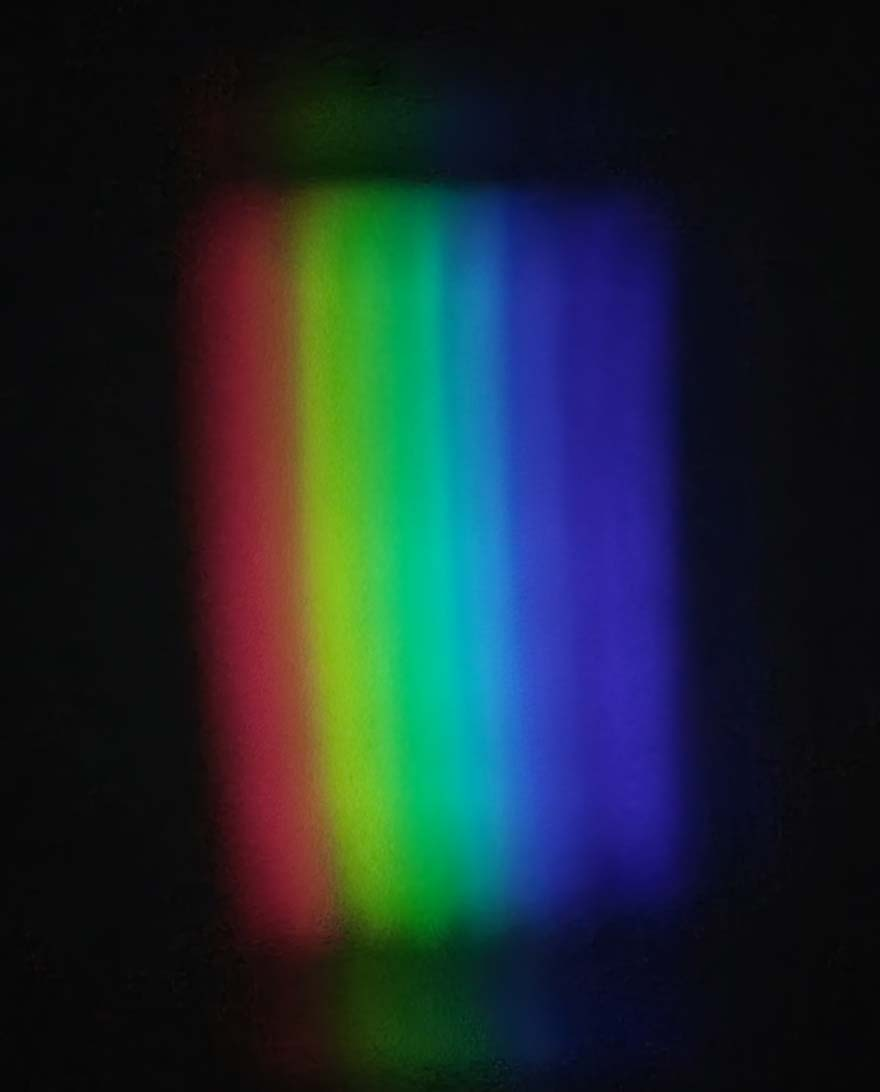
\includegraphics[width=0.6\linewidth]{nudes/rgb wand.jpg}
    \caption{Spektrallinien der einzelnen Farben der Quecksilberlampe reflektiert an der Laborwand}
    \label{fig:spektallinien Prisma}
\end{figure}

\noindent
Der Abstand $L$ vom Fernrohr zum Kollimator beträgt $(12.1 \pm 0.3)cm$, der Durchmesser $d$ des Kollimators beträgt $(1.4 \pm 0.2)cm$


\section{Auswertung und Unsicherheitsanalyse} %Nicht nur zahlen angeben ------------------------------
In der Auswertung werden zur erhöhten Genauigkeit durchgehend ungerundete Werte bis zu den Endergebnissen verwendet und nur zur Darstellung gerundet. \\
Zur Berechnung der Unsicherheiten wird, wenn nicht anders angegeben, die Größtunsicherheitsmethode verwendet.

\subsection{Gitter}
Aus den Messdaten aus Tabelle \ref{tab:Gitter v1} wird mit der Formel \ref{eq:Mittelwert} der Mittelwert berechnet. Die Bogenminuten werden noch in Grad umgerechnet mit der Formel: 

\begin{equation}
    \label{eq:Bogenwix}
    \centerline{$Grad = \frac{Bogenminuten}{60}$}
\end{equation}
Daraus ergeben sich für die Winkel $\varphi_{Links} = (41.05 \pm 0.02)$ Grad und für $\varphi_{Rechts} = (140.07 \pm 0.02) $ Grad. Die Unsicherheit $\Delta \varphi $ beträgt eine Bogensekunde = 0.02 Grad. 
\\
Mit der Formel
\begin{equation}
    \label{eq:formel für gitterwix}
    \centerline{$\varphi = \frac{\varphi_{Rechts} - \varphi_{Links}}{2}$}
\end{equation}
wird der Winkel $\varphi = (49.51 \pm 0.02) Grad$ berechnet und mit der Wellenlänge $\lambda = (5889.95 \pm 0.01)$ \AA, welche auf Seite 5 des Skriptes \cite{teachcenter2} angegeben ist, lässt sich mit Formel \ref{eq:Gitterkonstante}, $z=2$ weil die hinteren Spektrallinien gemessen wurden, und für die Unsicherheit die Formel 

\begin{equation}
    \label{eq:uns gitterkonstante}
    \centerline{$ \Delta g = \vert \frac{\partial g}{\partial \lambda} * \Delta \lambda \vert + \vert \frac{\partial g}{\partial \varphi} * \Delta \varphi \vert$}
\end{equation}

\noindent
die Gitterkonstante $g = (1.55 \pm 0.03) \mu m$ bestimmen. 
\\
\\
Für die Werte aus der Tabelle \ref{tab:Gitter v2} wird wieder der Mittelwert mit Formel \ref{eq:Mittelwert} berechnet. 
Der Winkel $\varphi$ wird wie zuvor mit der Formel \ref{eq:Bogenwix} und selber Unsicherheit berechnet. 

\begin{table}[H]
    \centering
    \caption{Gemittelter Winkel $\varphi$}
    \label{tab:gitterwinkel}
    \begin{tabular}{| l | l |}
        \hline
        Farbe & $\varphi$ [Grad] \\
        \hline
        Lila        & $ 42.13 \pm 0.02 $ \\
        Hellblau    & $ 48.58 \pm 0.02 $ \\
        Grün        & $ 54.06 \pm 0.02 $ \\
        Gelb        & $ 56.58 \pm 0.02 $ \\
        Rot         & $ 63.34 \pm 0.02 $ \\
        \hline
    \end{tabular}
\end{table}

\noindent
Durch die zuvor bestimmte Gitterkonstante $g = (1.55 \pm 0.03) \mu m$ kann mit der Formel \ref{eq:Gitterkonstante} ($z=2$) die Wellenlänge $\lambda$ berechnet werden. 
Für die Unsicherheit verwendet man die Formel

\begin{equation}
    \label{eq:uns wellenwix}
    \centerline{$ \Delta \lambda = \vert \frac{\partial \lambda}{\partial g} * \Delta g \vert + \vert \frac{\partial \lambda }{\partial \varphi} * \Delta \varphi \vert$}
\end{equation}

\noindent
und erhält dadurch die Unsicherheit der Wellenlänge $\Delta \lambda = \pm 0.04 nm$, welche für alle Werte gerundet die gleiche ist. 

\begin{table}[H]
    \centering
    \caption{Wellenlänge $\lambda$ der einzelnen Farben}
    \label{tab:wellenlänge gitter}
    \begin{tabular}{| l | l |}
        \hline
        Farbe & $\lambda$ [nm] \\
        \hline
        Lila        & $ 519.89 \pm 0.04 $ \\
        Hellblau    & $ 581.16 \pm 0.04 $ \\
        Grün        & $ 627.47 \pm 0.04 $ \\
        Gelb        & $ 646.86 \pm 0.04 $ \\
        Rot         & $ 692.62 \pm 0.04 $ \\
        \hline
    \end{tabular}
\end{table}

\noindent
Das Auflösungsvermögen wird durch die Formel \ref{eq:Auflösungsvermögen} berechnet. 
Die Größe $D = 1/570 = 0.001754 mm = 1.754 \mu m$ wird über den Kehrwert der Striche pro Milimeter gebildet, siehe Bild \ref{fig:gitterundprisma}. Mit der zuvor berechneten Gitterkonstante $g$ kann man das Auflösungsvermögen berechnen. 
Setzt man die Werte in die Formel \ref{eq:Auflösungsvermögen} ein, so erhält man für $\lambda / \Delta \lambda = (2.27 \pm 0.05)$. 
Für die Unsicherheit wurde die Formel

\begin{equation}
    \label{eq:uns Auflösungsvermögen}
    \centerline{$ \Delta \frac{\lambda}{\Delta \lambda} = \vert \frac{\partial}{\partial g} * \Delta g \vert$}
\end{equation}

\noindent
verwendet. 

\subsection{Prisma}
Für die Werte aus der Tabelle \ref{tab:Prisma} für den brechende Winkel $\gamma$ wird der Mittelwert mit der Formel \ref{eq:Mittelwert} berechnet. 
Der Winkel $\gamma$ wird mit der Formel

\begin{equation}
    \label{eq:formel für prismawix}
    \centerline{$\gamma = \gamma_{Rechts} - \gamma_{Links}$}
\end{equation}

\noindent
berechnet. Daraus erhält man den Winkel $\gamma = (59.40 \pm 0.02)$ des Prisma. 
\\
\\
Durch die Formel \ref{eq:Ablenkungswinkel} und den Messwerten aus Tabelle \ref{tab:Prisma v2} lässt sich der minimale Brechungswinkel $\delta$ berechnen. 
Die Unsicherheit $\Delta \delta$ beträgt eine Bogenminute = 0.02 Grad. 

\begin{table}[H]
    \centering
    \caption{Brechungswinkel $\delta$ der einzelnen Farben}
    \label{tab:delta scheiß}
    \begin{tabular}{| l | l |}
        \hline
        Farbe & $\delta$ [Grad] \\
        \hline
        Lila        & $ 29.85 \pm 0.02 $ \\
        Hellblau    & $ 29.85 \pm 0.02 $ \\
        Grün        & $ 29.84 \pm 0.02 $ \\
        Gelb        & $ 29.80 \pm 0.02 $ \\
        Rot         & $ 29.64 \pm 0.02 $ \\
        \hline
    \end{tabular}
\end{table}

\noindent
Mit der Formel \ref{eq:Brechungsindex} und dem zuvor berechneten brechenden Winkel $\gamma = (59.40 \pm 0.02)$ des Prisma lassen sich noch die einzelnen Brechungsindizes berechnen. 
Für die Unsicherheit verwendet man die Formel

\begin{equation}
    \label{eq:uns n}
    \centerline{$ \Delta n = \vert \frac{\partial n}{\partial \gamma} * \Delta \gamma \vert + \vert \frac{\partial n }{\partial \delta} * \Delta \delta \vert$}
\end{equation}

\noindent
und erhält für $\Delta n = 0.0004$. Die Unsicherheit ist gerundet für die einzelnen Farben die gleiche. 

\begin{table}[H]
    \centering
    \caption{Brechungsindizes $n$}
    \label{tab:delta n}
    \begin{tabular}{| l | l |}
        \hline
        Farbe & $n$ [1] \\
        \hline
        Lila        & $ 1.4178 \pm 0.0004 $ \\
        Hellblau    & $ 1.4178 \pm 0.0004 $ \\
        Grün        & $ 1.4177 \pm 0.0004 $ \\
        Gelb        & $ 1.4172 \pm 0.0004 $ \\
        Rot         & $ 1.4152 \pm 0.0004 $ \\
        \hline
    \end{tabular}
\end{table}

\begin{figure}[H]
    \centering
    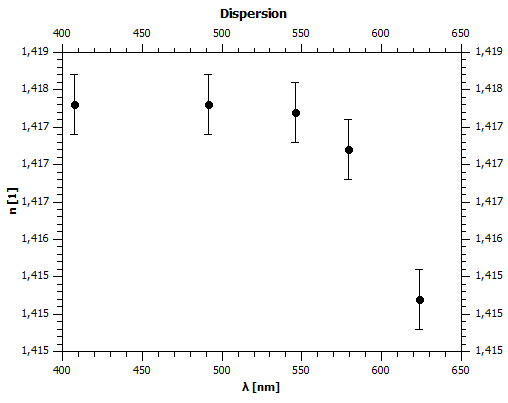
\includegraphics[width=0.6\linewidth]{nudes/Dispersion.png}
    \caption{Brechungsindizes $n$ aus der Tabelle \ref{tab:delta n}. Die Wellenlänge $\lambda$ wurde auf Seite 5 des Prisma Skriptes \cite{teachcenter2} bereitgestellt. Die Unsicherheit der Wellenlänge $\lambda$ wurde nicht angebeben, da der Wert sehr klein ist, und im Plot nicht sichtbar wäre.}
    \label{fig:Dispersion Prisma}
\end{figure}

\noindent
Das Auflösungsvermögen $\lambda / \Delta \lambda$ des Prismas ist je nach Wellenlänge $\lambda$ unterschiedlich. 
In diesem Fall wird das Auflösungsvermögen $\lambda / \Delta \lambda$  für eine gelbe Linie mit der Formel \ref{eq:Auflösungsvermögen Prisma} berechnet. 
Die Steigung der Dispersion beträgt laut qtiPlot $(-9.9 \pm -2.4 )\mu$. 
Für $t$ wird der Wert des Durchmessers des Kollimators verwendet.  
Setzt man die Werte in die vorher genannte Formel ein, so kommt man auf ein Auflösungsvermögen von $\lambda / \Delta \lambda = (0.14 \pm 0.05)$. 
Für die Unsicherheit wird folgende Formel verwendet. 

\begin{equation}
    \label{eq:uns Auflösungsvermögen Prisma}
    \centerline{$ \Delta \frac{\lambda}{\Delta \lambda} = \vert \frac{\partial}{\partial D} * \Delta D \vert + \vert \frac{\partial}{\partial t} * \Delta t \vert$}
\end{equation}

\section{Diskussion} %diskussion der Unsicherheiten und Ergebnisse und evtl. verlgeich mit Literatur ------------------------------
Die Brechung und Beugung des Lichts ist ein wichtiger Bestandteil der Optik. Sie erklären zusammenhänge wie Wellenlänge der einzelnen Farben des sichtbaren Lichtes sowie Brechende Winkel der Geometrischen Instrumente. 
Doch wie bei allen Experimenten ist auch dieses nicht von Fehlern verschont. 

\subsection{Gitter}
Ein optisches Gitter besteht aus mehreren Spalten. 
Durch die Spalten wird das Licht gebeugt. 
Die Aufgabe mit dem Gitter war es, die Gitterkonstante zu bestimmen. 
Vergleicht man diesen Wert mit dem auf dem Gitter aufgedruckten Wert von 570/mm, was im umkehrschluss durch den Kehrwert eine Gitterkonstante von $g=(1.76)\mu m$ ergibt, lässt darauf schließen, dass bei den Messungen ein Fehler entstanden ist. 
Es lässt sich daraus schließen, dass bei der Messung der Winkel ein Fehler aufgetreten ist. 
\\
\\
Bei dem zweiten Teilversuches mit dem Gitter wurden die Wellenlängen der verschiedenen sichtbaren Farben berechnet. 
In der Folgenden Tabelle werden die berechneten Wellenlängen des sichtbaren Lichtes mit Literaturwerten verglichen. 

\begin{table}[H]
    \centering
    \caption{Wellenlängen $\lambda$ sichtbares Licht }
    \label{tab:literatur wellenlänge}
    \begin{tabular}{| l | l | l |}
        \hline
        Farbe & Literaturwert \cite{wiki1} [nm] & Berechnete Werte [nm]\\
        \hline
        Lila        & 380 - 430 & $ 519.89 \pm 0.04 $ \\
        Hellblau    & 430 - 490 & $ 581.16 \pm 0.04 $ \\
        Grün        & 490 - 570 & $ 627.47 \pm 0.04 $ \\
        Gelb        & 570 - 600 & $ 646.86 \pm 0.04 $ \\
        Rot         & 640 - 780 & $ 692.62 \pm 0.04 $ \\
        \hline
    \end{tabular}
\end{table}

\noindent
Dabei erkennt man, dass die Wellenlänge der roten Farbe den zu erwartenden Wert entspricht. 
Bei der Wellenlänge der gelben Farbe sieht man bereits erste Abweichungen der Vergleichswerte. Die berechneten Werte liegen im Bereich oranger Farbe, was eine Wellenlänge von 600-640 nm hat. 
Bei den restlichen Wellenlängen sind offenbar systematische Fehler entstanden, da alle Werte höher sind als die Vergleichswerte. Eine mögliche Ursache wäre die Positionierung des Gitters. 
Durch eine nicht genau zentrale Positionierung des Gitters zwischen Kollimator und Fernrohr kann der beobachtete Lichtstrahl weiter seitlich erscheinen, was im Anschluss auf ein falsches Ablesen des Winkels $\varphi$ führt.
Bei erneuter Versuchsdurchführung sollte darauf geachtet werden, dass das Gitter genau Mittig plaziert wird. 

\subsection{Prisma}
Im zweiten Teil des Experimentes wird der brechende Winkel eines Prismas bestimmt. Der Winkel $\gamma = (59.40 \pm 0.02)$ entspricht größtenteils den zu erwartenden Wert von 60 Grad. 
Da der Prisma die Grundform eines gleichseitigen Dreiecks hat, muss der brechende Winkel 60 Grad haben. 
\\
\\
Im zweiten Teilversuch des Prismas wird die Dispersionskurve \ref{fig:Dispersion Prisma} bestimmt. 
Der berechnete Wert lässt darauf schließen, dass es sich bei dem Material des Prismas um Kronglas handelt. 

\begin{figure}[H]
    \centering
    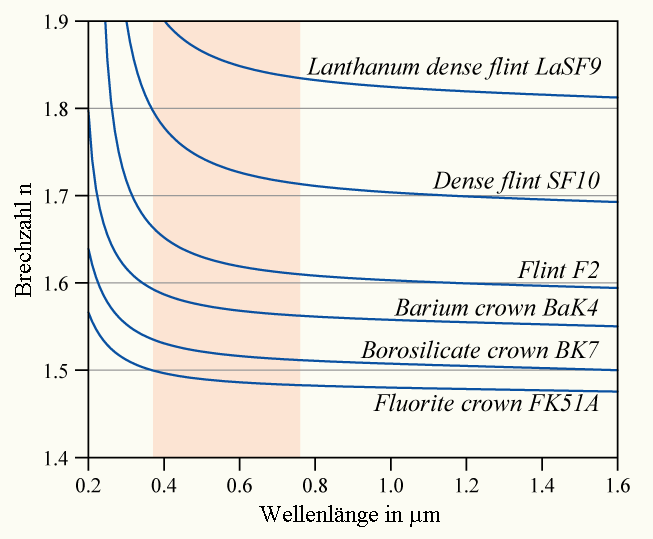
\includegraphics[width=0.6\linewidth]{nudes/Dispersionskurve.png}
    \caption{Dispersionskurve mit Materialien \cite{wiki2}}
    \label{fig:Literatur Prisma}
\end{figure}

\noindent
Da die berechneten Werte verglichen mit den Literaturwerten sehr realistisch erscheinen, kann auf eine fehlerfreie Durchführung geschlossen werden. 

\section{Zusammenfassung} %klare, übersichtliche vollständige beantwortung der Aufgabenstellung ------------------------------
Hier nocheinmal die in der Aufgabenstellung angegebenen Werte zusammengefasst. 

\subsection{Gitter}
Gitterkonstante  $g = (1.55 \pm 0.03)\mu m$ \\
Wellenlänge $\lambda$

\begin{table}[H]
    \centering
    \caption{Wellenlänge $\lambda$ der einzelnen Farben}
    \label{tab:zus wellenlänge gitter}
    \begin{tabular}{| l | l |}
        \hline
        Farbe & $\lambda$ [nm] \\
        \hline
        Lila        & $ 519.89 \pm 0.04 $ \\
        Hellblau    & $ 581.16 \pm 0.04 $ \\
        Grün        & $ 627.47 \pm 0.04 $ \\
        Gelb        & $ 646.86 \pm 0.04 $ \\
        Rot         & $ 692.62 \pm 0.04 $ \\
        \hline
    \end{tabular}
\end{table}

\noindent
Auflösungsvermögen $\lambda / \Delta \lambda = (2.27 \pm 0.05)$

\subsection{Prisma}
Brechender Winkel $\gamma = (59.40 \pm 0.02)$ \\
Minimale Brechungswinkel $\delta$ \\

\begin{table}[H]
    \centering
    \caption{Brechungswinkel $\delta$ der einzelnen Farben}
    \label{tab:zus delta scheiß}
    \begin{tabular}{| l | l |}
        \hline
        Farbe & $\delta$ [Grad] \\
        \hline
        Lila        & $ 29.85 \pm 0.02 $ \\
        Hellblau    & $ 29.85 \pm 0.02 $ \\
        Grün        & $ 29.84 \pm 0.02 $ \\
        Gelb        & $ 29.80 \pm 0.02 $ \\
        Rot         & $ 29.64 \pm 0.02 $ \\
        \hline
    \end{tabular}
\end{table}

\noindent
Brechungsindizes $n$ \\

\begin{table}[H]
    \centering
    \caption{Brechungsindizes $n$}
    \label{tab:zus delta n}
    \begin{tabular}{| l | l |}
        \hline
        Farbe & $n$ [1] \\
        \hline
        Lila        & $ 1.4178 \pm 0.0004 $ \\
        Hellblau    & $ 1.4178 \pm 0.0004 $ \\
        Grün        & $ 1.4177 \pm 0.0004 $ \\
        Gelb        & $ 1.4172 \pm 0.0004 $ \\
        Rot         & $ 1.4152 \pm 0.0004 $ \\
        \hline
    \end{tabular}
\end{table}

\noindent
Auflösungsvermögen $\lambda / \Delta \lambda = (0.14 \pm 0.05)$

\printbibliography[heading=bibintoc]

\begin{figure}[H]
    \centering
    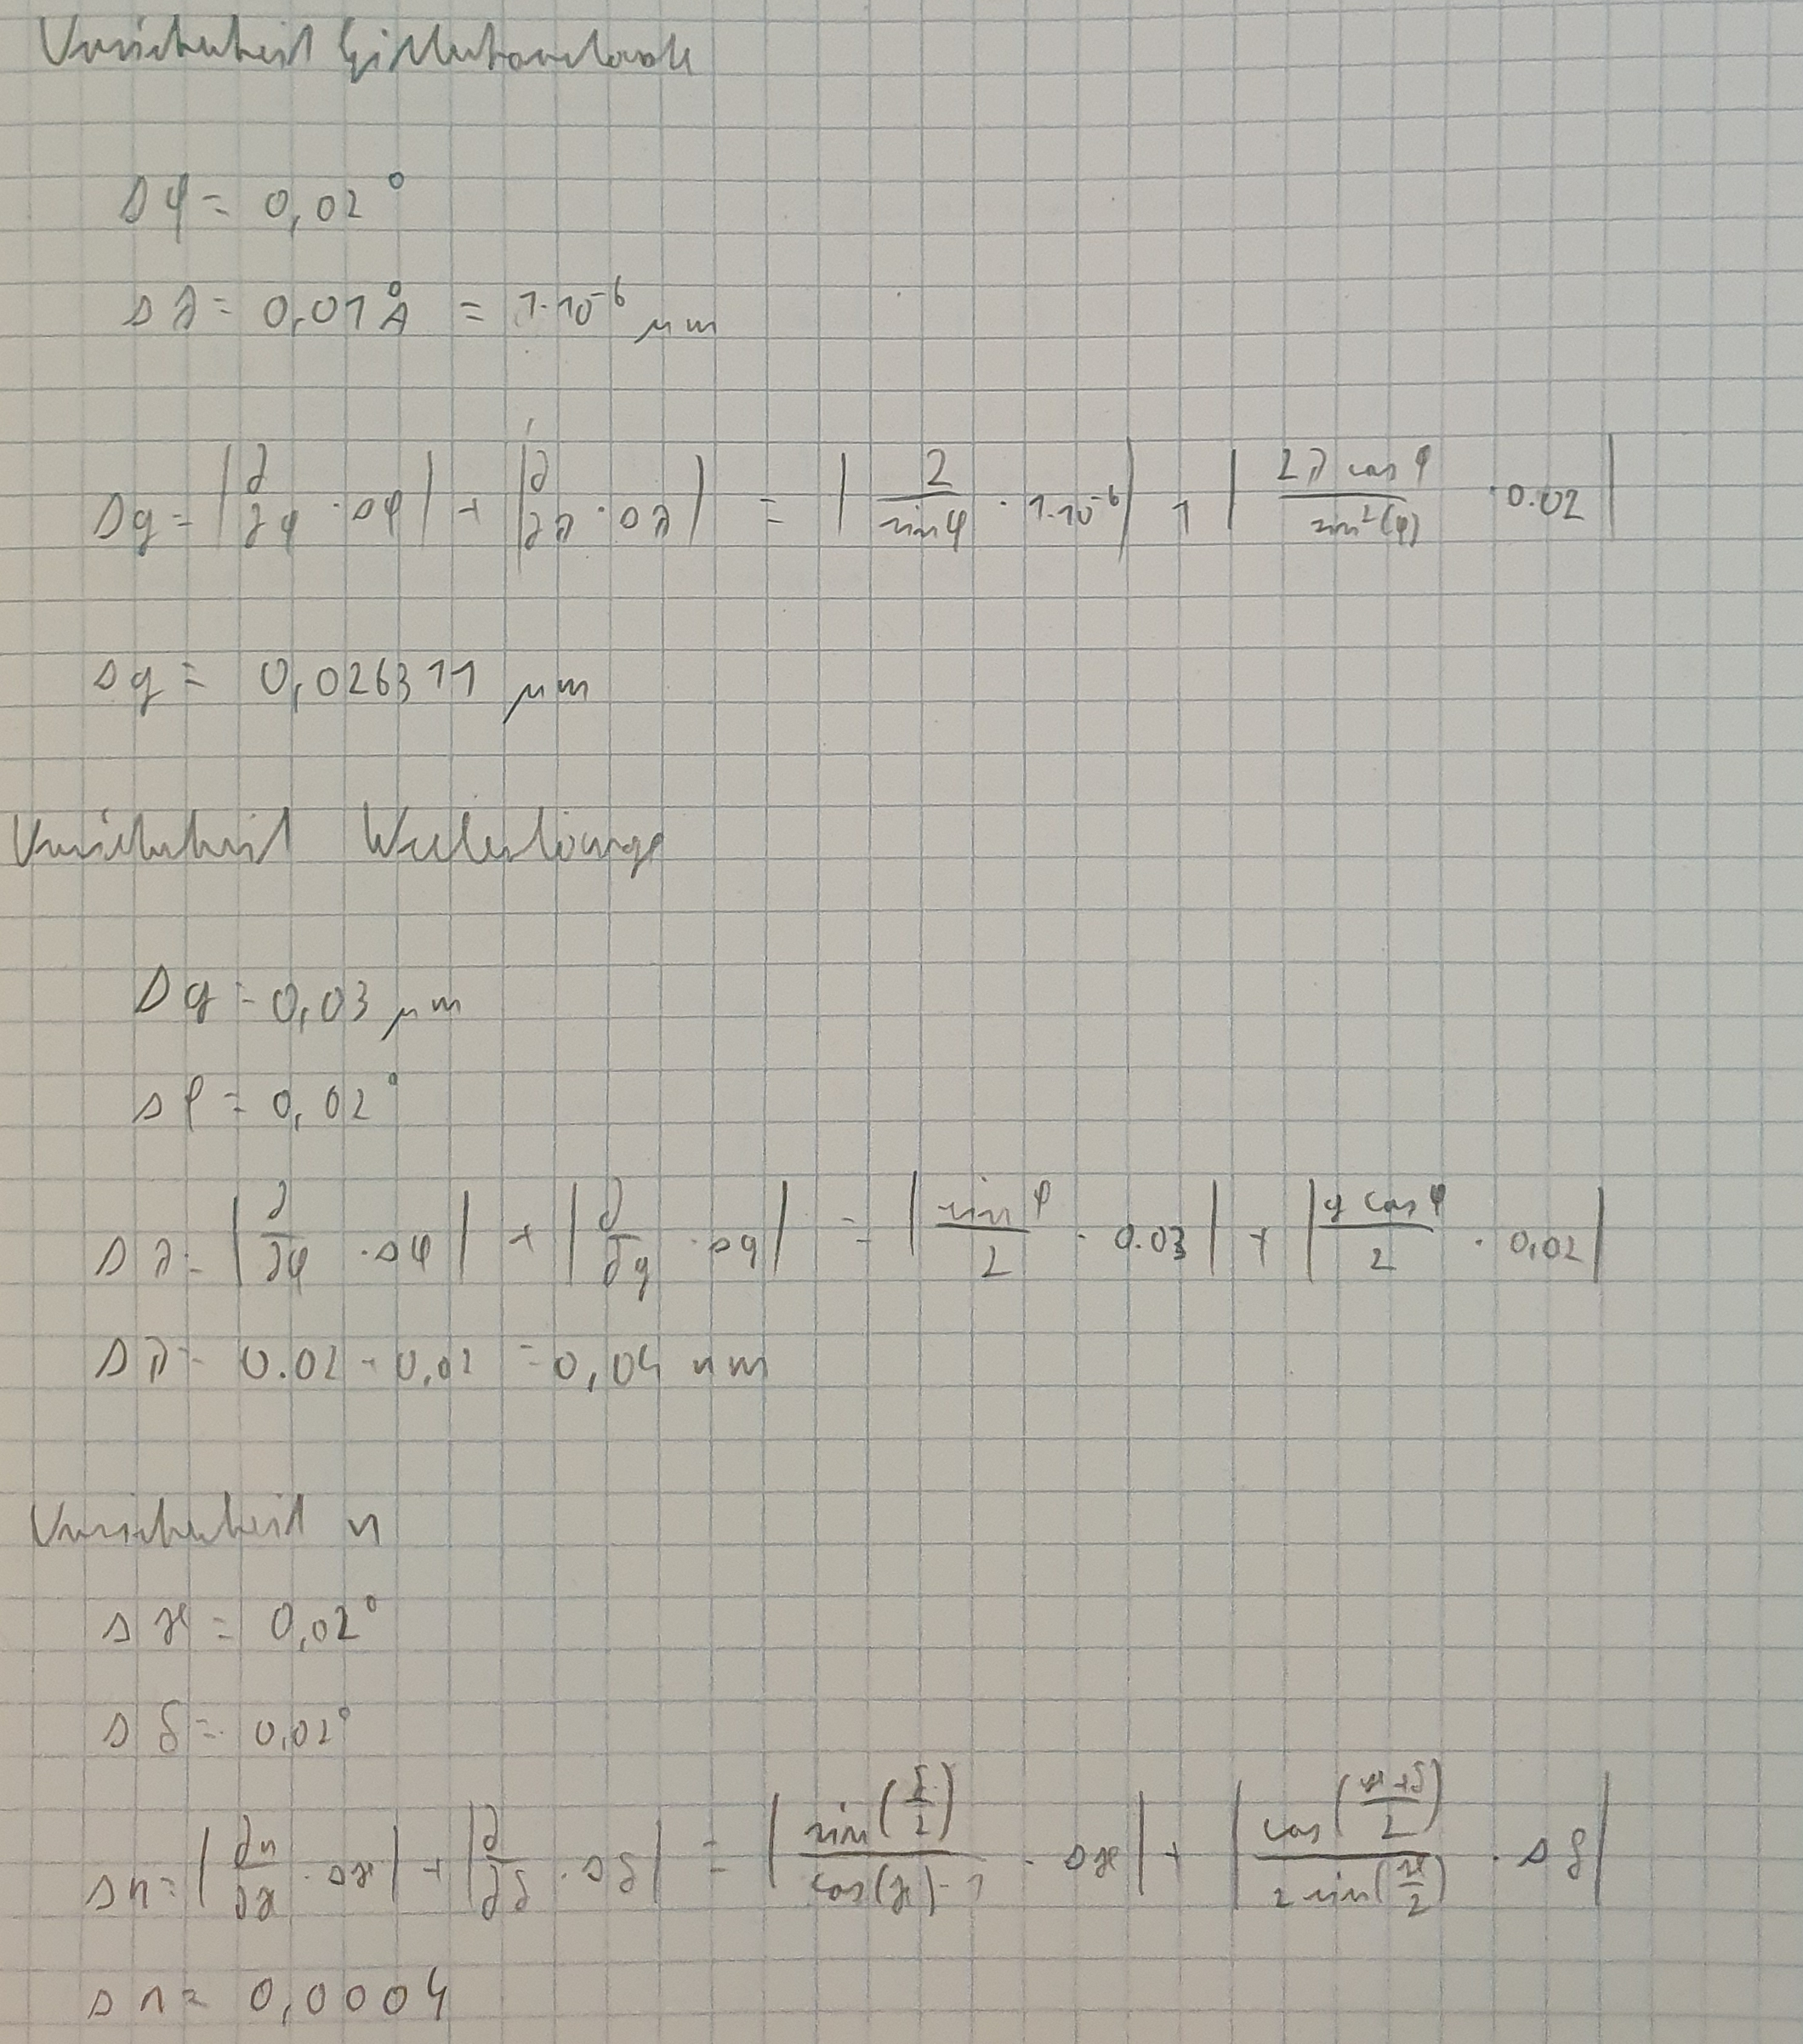
\includegraphics[width=1\linewidth]{nudes/uns2.jpg}
    \caption{Unsicherheitsrechnung}
    \label{fig:uns1}
\end{figure}

\begin{figure}[H]
    \centering
    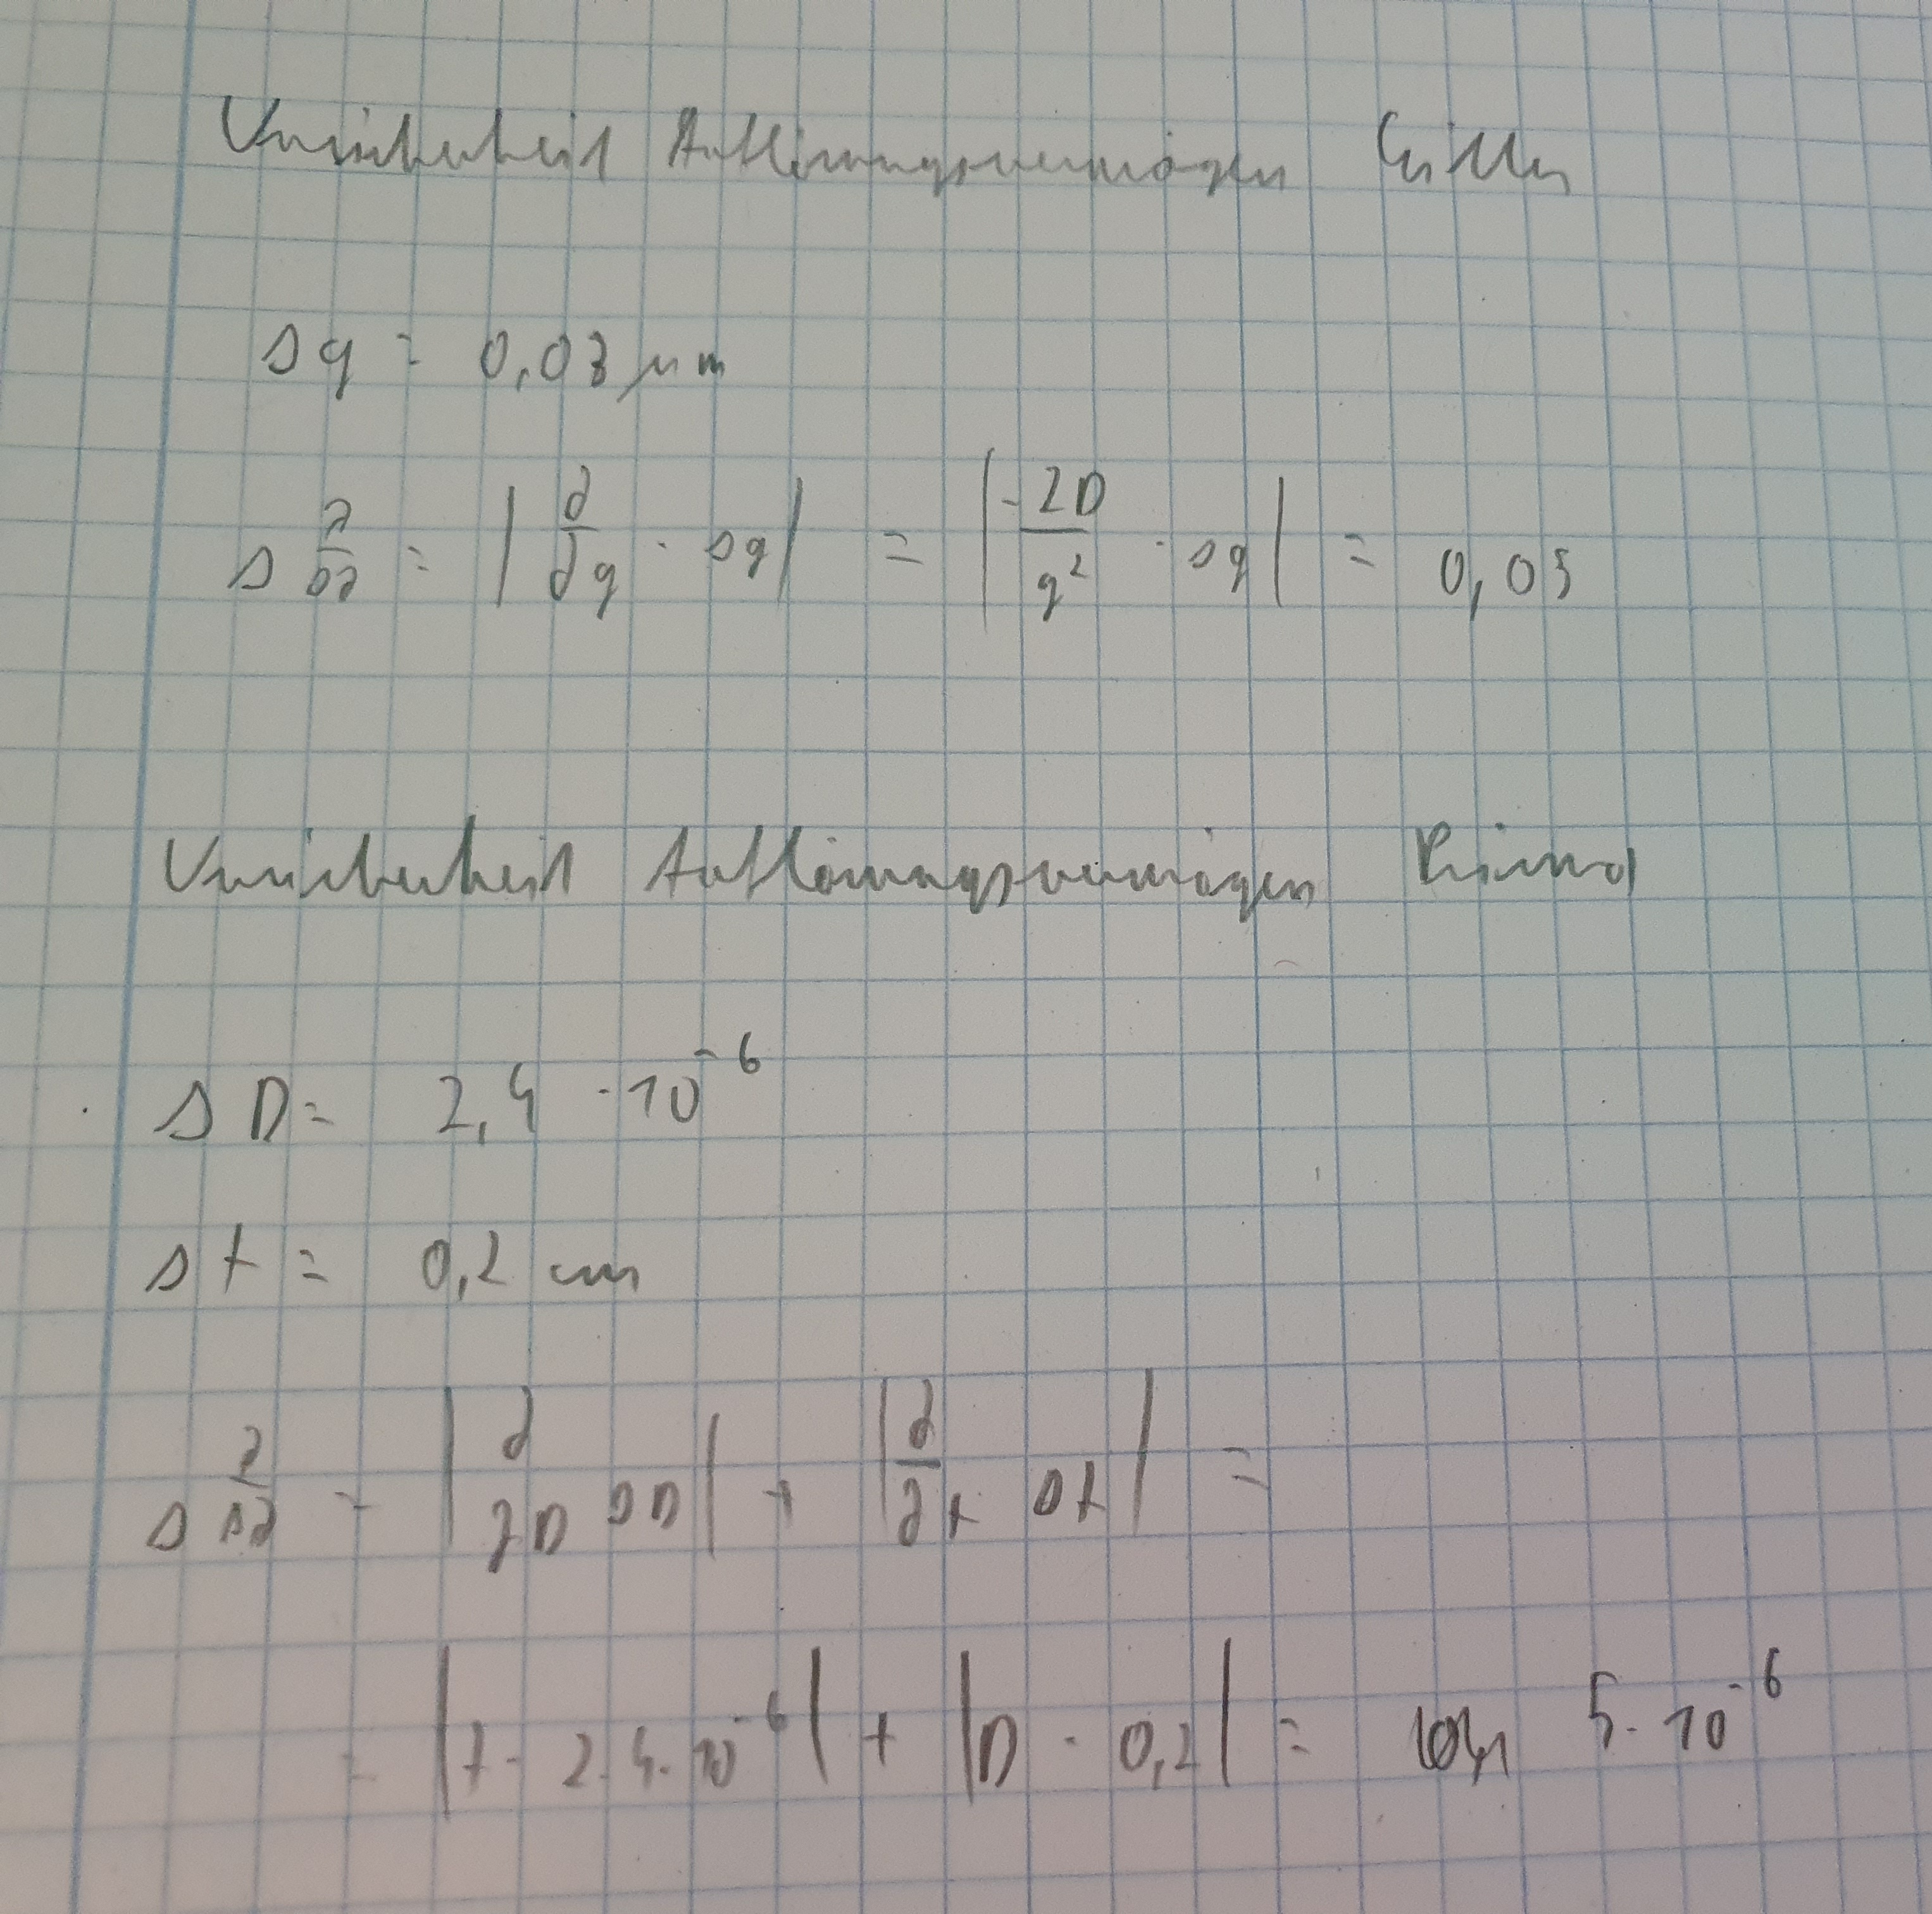
\includegraphics[width=1\linewidth]{nudes/uns1.jpg}
    \caption{Unsicherheitsrechnung}
    \label{fig:uns2}
\end{figure}

\end{document}
